\section{基于多重校验的时间隐通道评估}
\label{chap:hash:result}

基于多重校验的时间隐通道评估,主要由抗检测能力测试、鲁棒性测试、传输性能测试及构建代价测试及部分组成。其中,抗检测能力测试按照\nref{chap:analyze:statistical}中提出的检测方法,由IPD测试、突发丢包长度测试及区间丢包数测试组成。鲁棒性测试,主要评估不同场景下,时间隐通道在不同参数配置时的平均误码率。传输性能测试,评估不同参数配置下的传输速率,测试时间隐通道的数据传输能力。

\subsection{评估环境及参数}
\label{chap:hash:result:parameters}

该时间隐通道的参数包括$L_{Codeword}$、$L_{HASH}$、$L_{CRC}$、$R$及$M_{cols}$,其中,$L_{Codeword}$代表了时间隐通道的主动丢包密度。参数$L_{HASH}$及$L_{CRC}$与鲁棒性密切相关,分别代表了码字中嵌入的HASH校验块的位数,以及码字中嵌入的CRC校验块的位数。参数$R$代表了基于HASH的码字间校验复位周期,复位周期过长会导致可行解数量过多,影响解调过程的执行效率。参数$M_{cols}$代表了映射矩阵的列数,列数越多则矩阵规模越大,数据包序号与符号的对应关系越复杂。

\insertTable{
	\begin{table}
      \centering
      \caption{测试环境信息表}
      \label{tab:5:result:environment}
          \begin{tabular*}{0.9\textwidth}{@{\extracolsep{\fill}}cc}
            \toprule
            类型 & 详细信息 \\
            \midrule
            PC平台 & I5-9400,DDR4 16GB \\
            软件版本 & Windows 7,QT 5.9.5,python 3.6;Ubuntu 16.04,mysql 5.7 \\
            数据集 & VoLTE抓包结果,随机噪声 \\
            \bottomrule
          \end{tabular*}
    \end{table}
}

评估实验的软硬件环境如表\nref{tab:5:result:environment},测试数据集包括VoLTE抓包得到的结果,以及随机生成的网络噪声,隐蔽消息同样随机生成。所有的数据均存储到mysql数据库中,基于QT实现时间隐通道处理逻辑,最终对比调制与解调结果。基于python脚本,将抓包结果还原为视频数据,并评估调制前后的视频质量,得到隐通道构建代价测试结果。

\insertTable{
	\begin{table}
      \centering
      \caption{基于多重校验的时间隐通道参数范围}
      \label{tab:5:parameters}
          \begin{tabular*}{0.5\textwidth}{@{\extracolsep{\fill}}cc}
            \toprule
            参数名称 & 取值范围 \\
            \midrule
            $L_{Codewrod}$ & 7,\ 8,\ 9,\ 10,\ 11 \\  
            $L_{HASH}$ & 2,\ 3,\ 4,\ 5 \\
            $L_{CRC}$ & 2,\ 3,\ 4,\ 5 \\
            $R$ & 1,\ 2,\ 3 \\
            $M_{cols}$ & 9,\ 18,\ 27,\ 36,\ 45 \\
            \bottomrule
          \end{tabular*}
    \end{table}
}

该时间隐通道的测试参数如表\nref{tab:5:parameters},其中,$L_{Codeword}$、$L_{HASH}$、$L_{CRC}$及$BL$的关系如公式(\nref{equ:5:codeword-length})。为得到有效的评估结果,在测试数据集方面,包含了Excellent场景及Good场景的抓包结果,以及丢包率在0.5\%、1\%、2\%及5\%的随机噪声。

\subsection{抗检测能力测试}
\label{chap:hash:result:undetectability}

\insertFigure{
	\begin{figure}
        \centering
        \subfigure[Excellent场景的CDF]{
            \label{fig:5:result:ipd:cdf:excellent}
            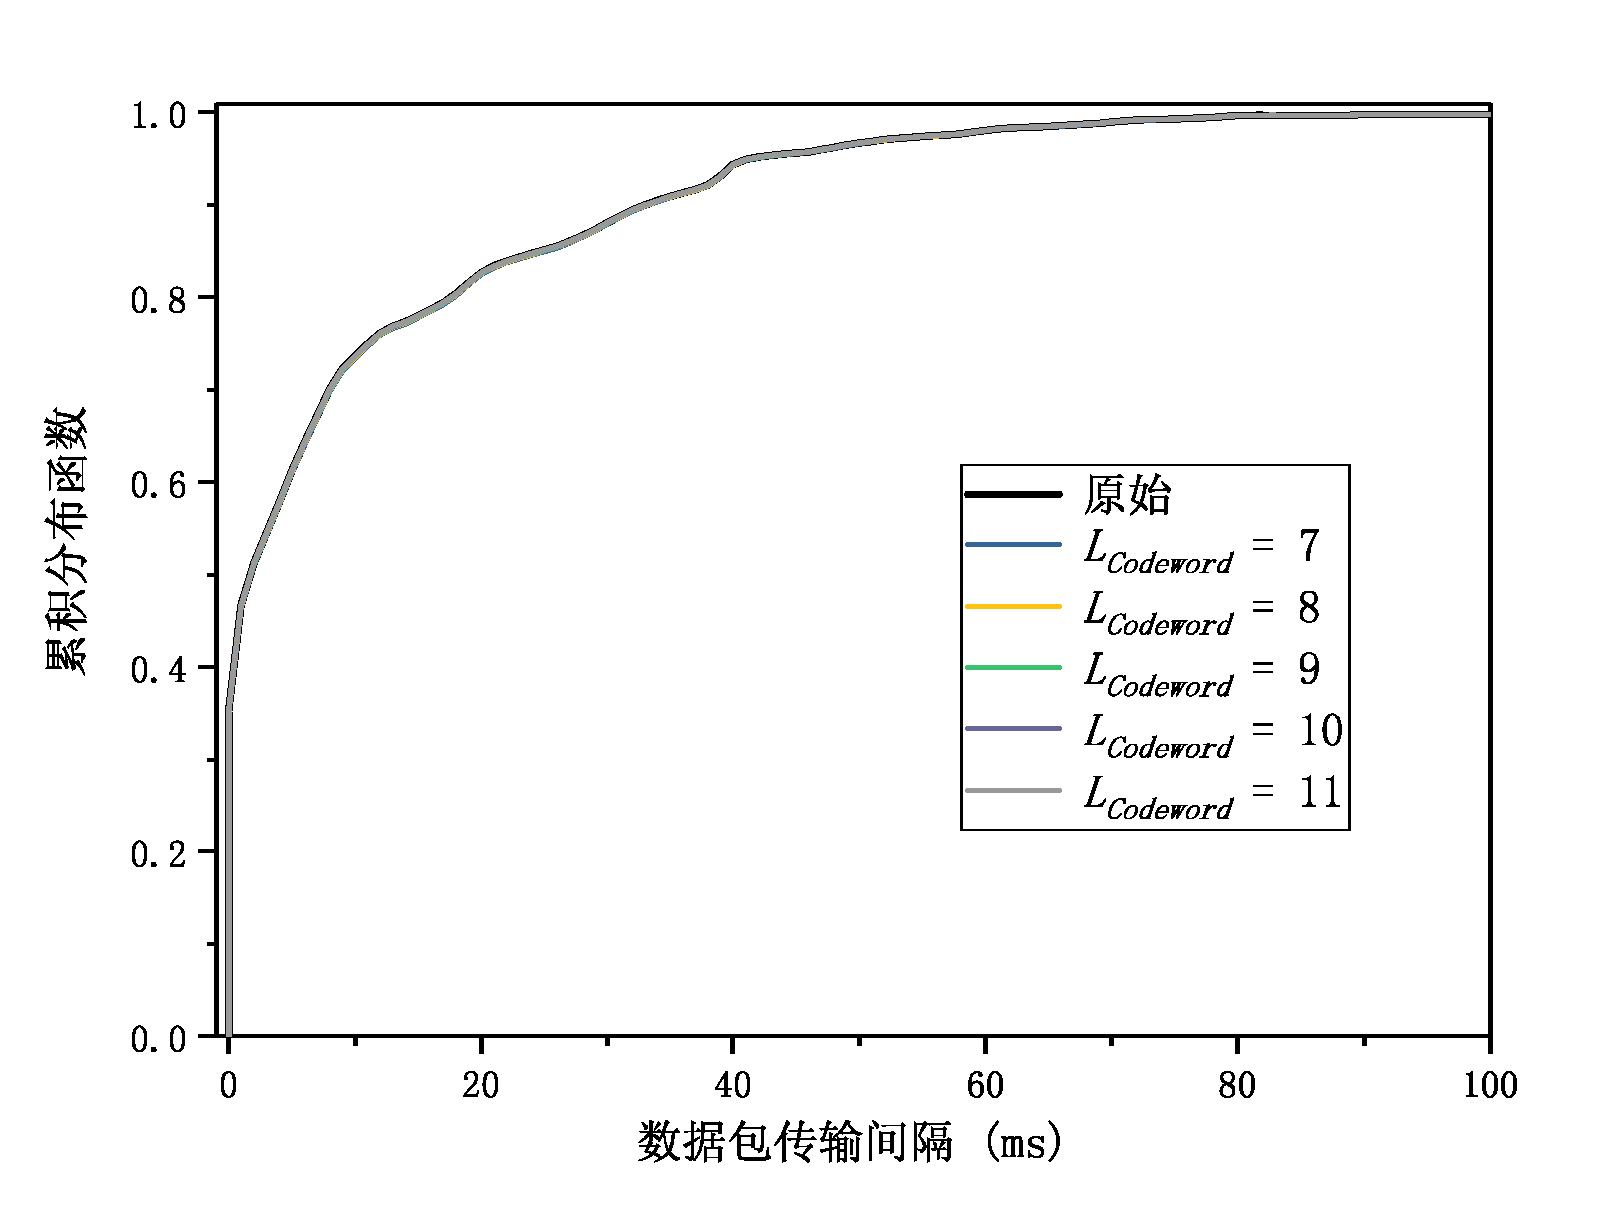
\includegraphics[width=0.48\textwidth]{chapters/chapter5/figures/ipd-cdf-excellent.pdf}
        }
        \subfigure[Good场景的CDF]{
            \label{fig:5:result:ipd:cdf:good}
            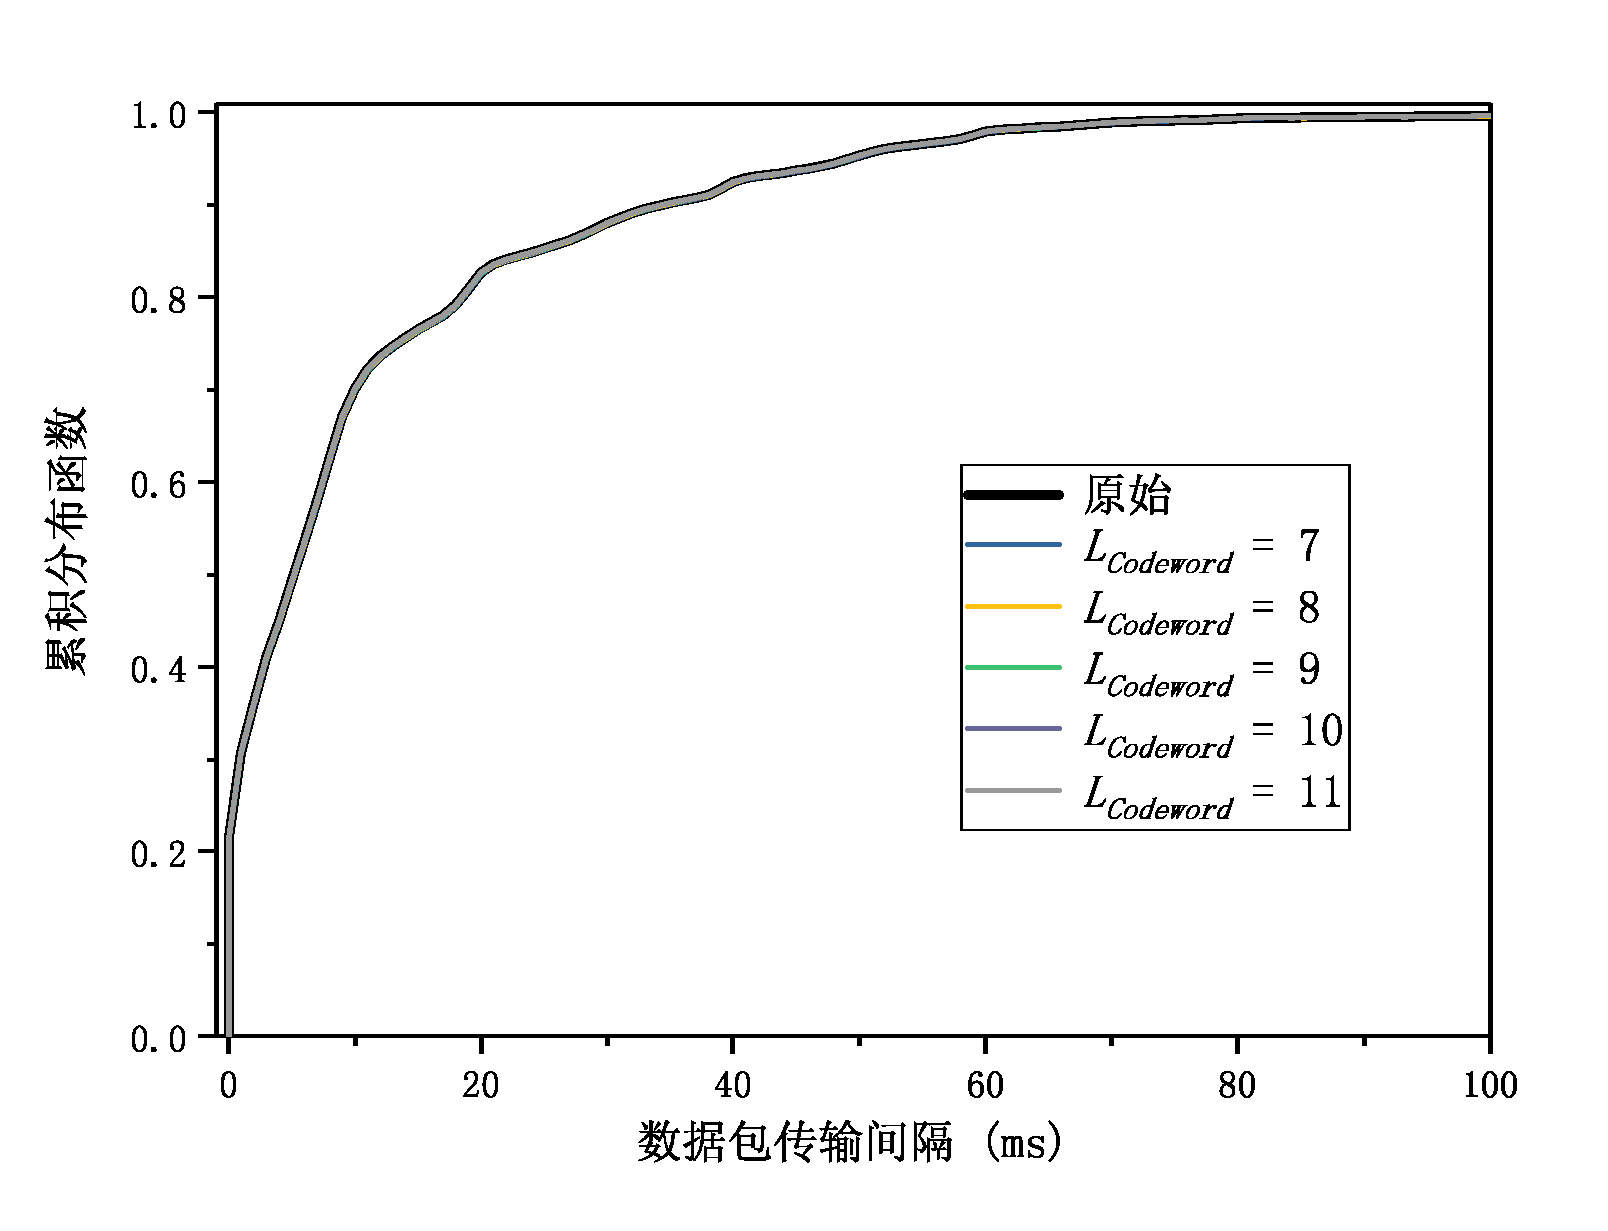
\includegraphics[width=0.48\textwidth]{chapters/chapter5/figures/ipd-cdf-good.pdf}
        }
        \caption{IPD分布的CDF曲线}
        \label{fig:5:result:ipd:cdf}
    \end{figure}
    
    \begin{figure}
        \centering
        \subfigure[Excellent场景的CDF]{
            \label{fig:5:result:burst:cdf:excellent}
            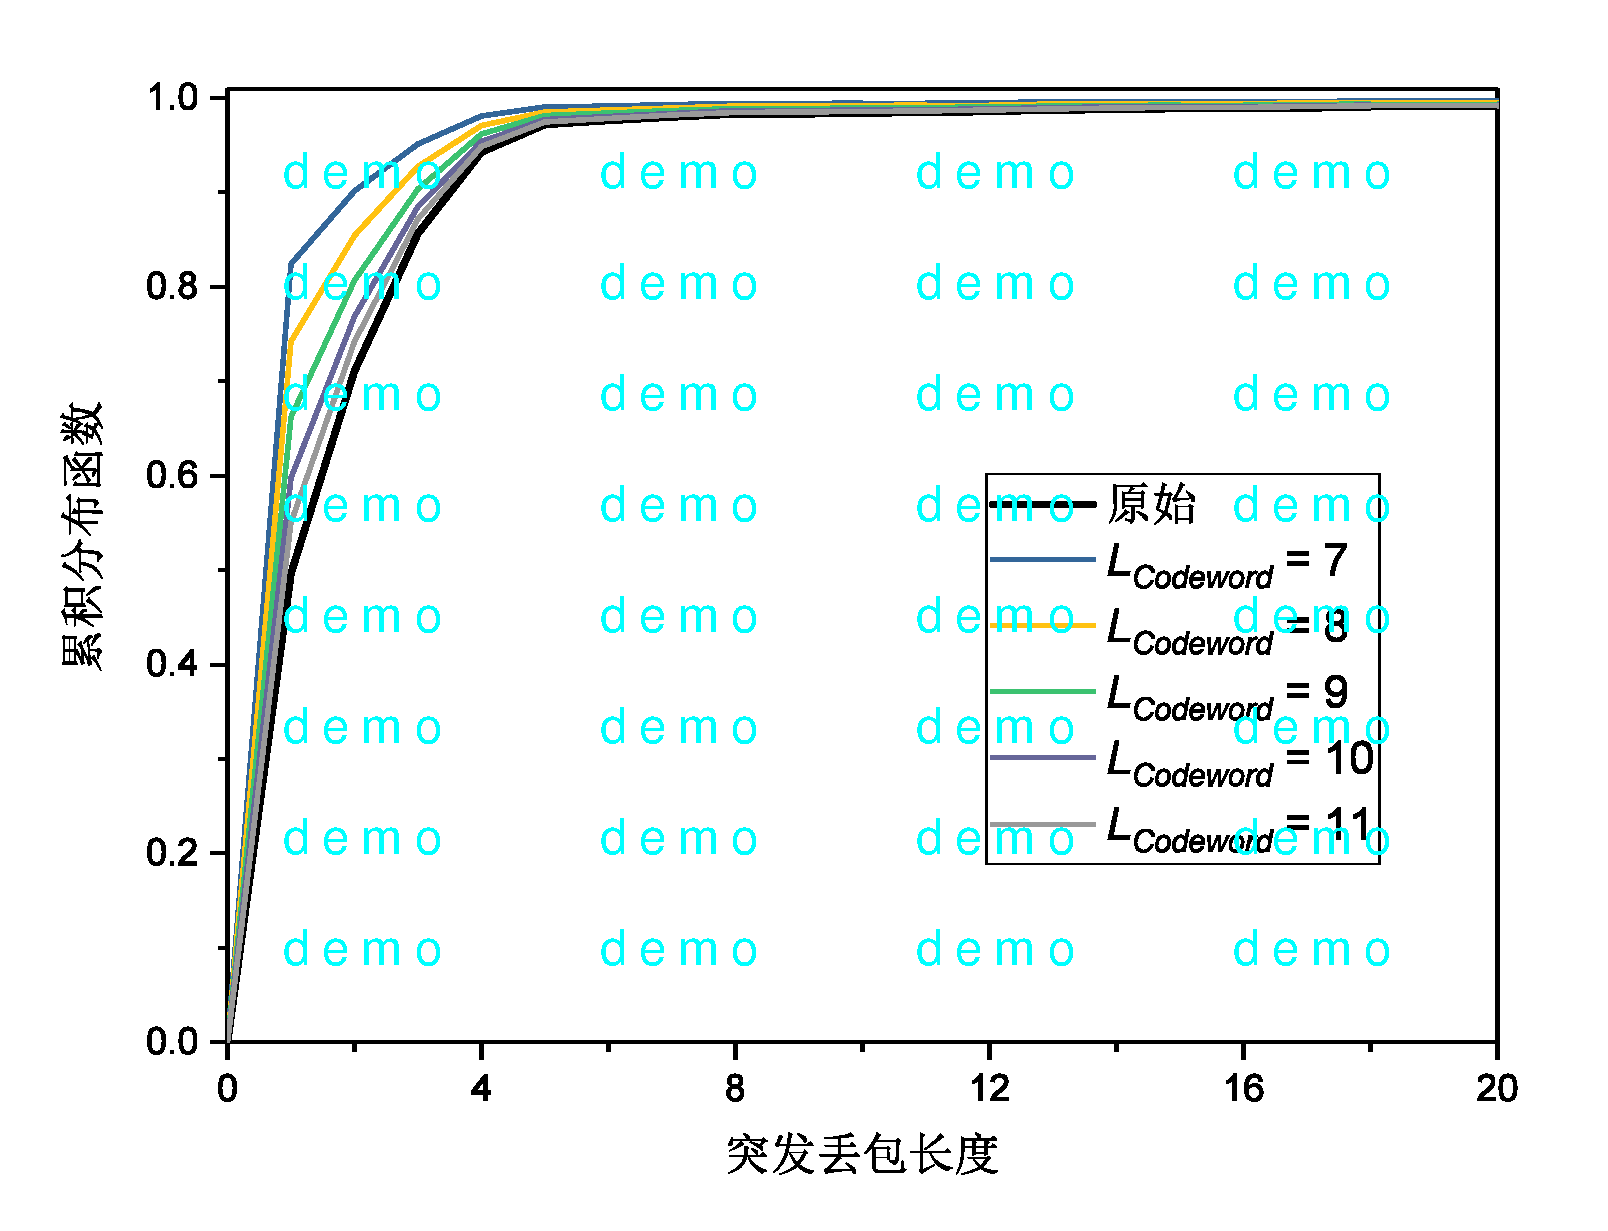
\includegraphics[width=0.48\textwidth]{chapters/chapter5/figures/burst-cdf-excellent.pdf}
        }
        \subfigure[Good场景的CDF]{
            \label{fig:5:result:burst:cdf:good}
            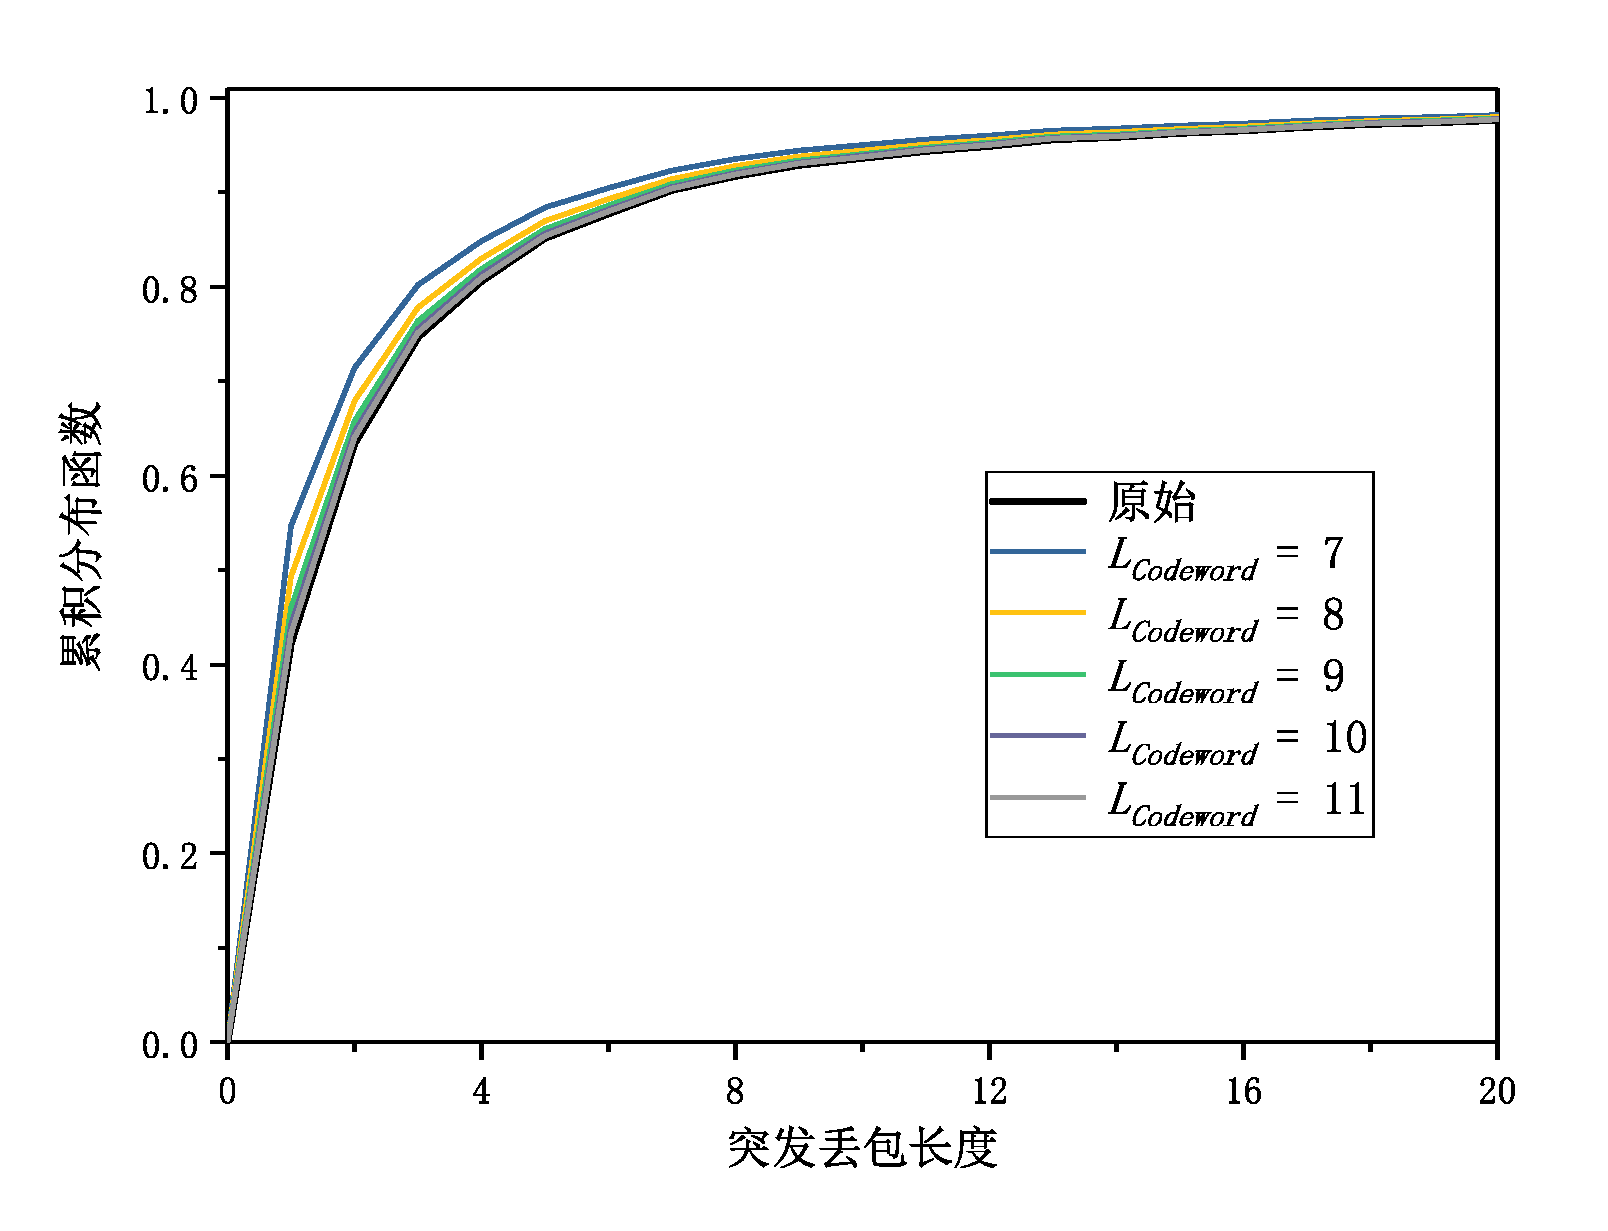
\includegraphics[width=0.48\textwidth]{chapters/chapter5/figures/burst-cdf-good.pdf}
        }
        \caption{突发丢包长度的CDF曲线}
        \label{fig:5:result:burst:cdf}
    \end{figure}
    
    \begin{figure}
        \centering
        \subfigure[窗口100时Excellent场景的CDF]{
            \label{fig:5:result:win100:cdf:excellent}
            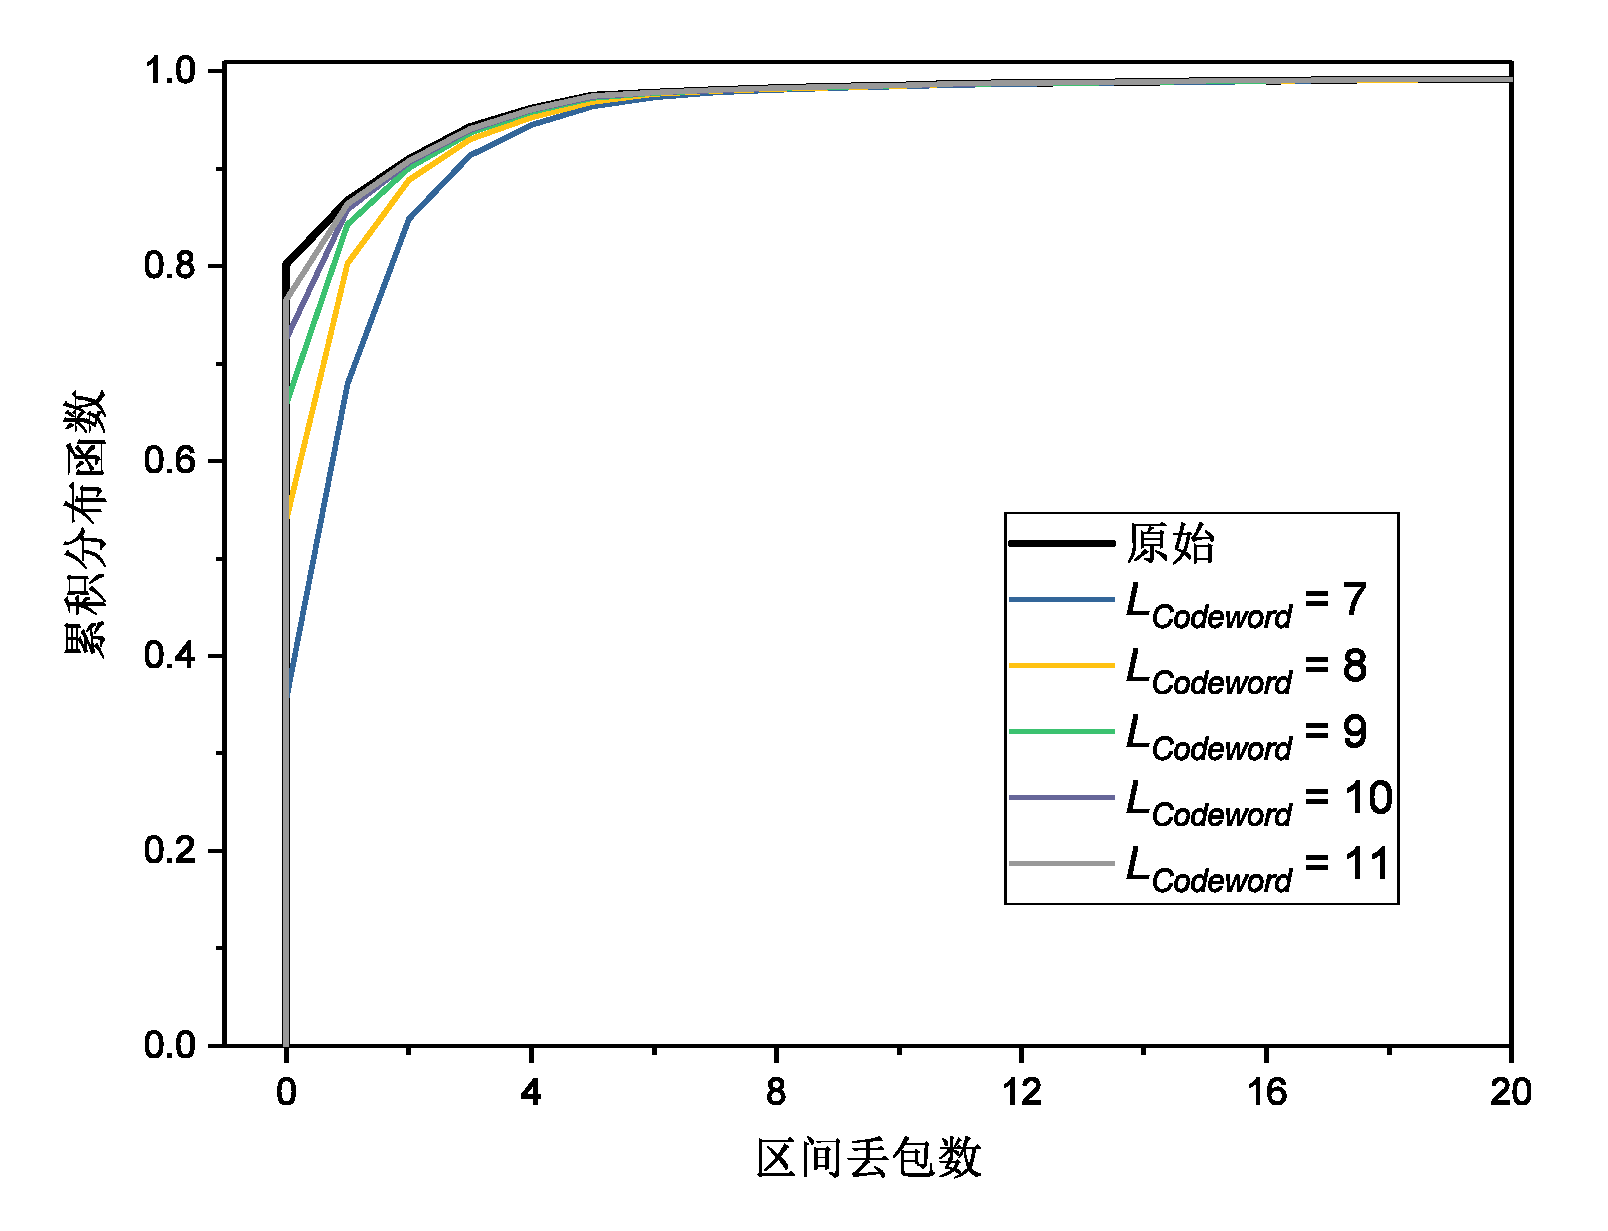
\includegraphics[width=0.48\textwidth]{chapters/chapter5/figures/win100-cdf-excellent.pdf}
        }
        \subfigure[窗口100时Good场景的CDF]{
            \label{fig:5:result:win100:cdf:good}
            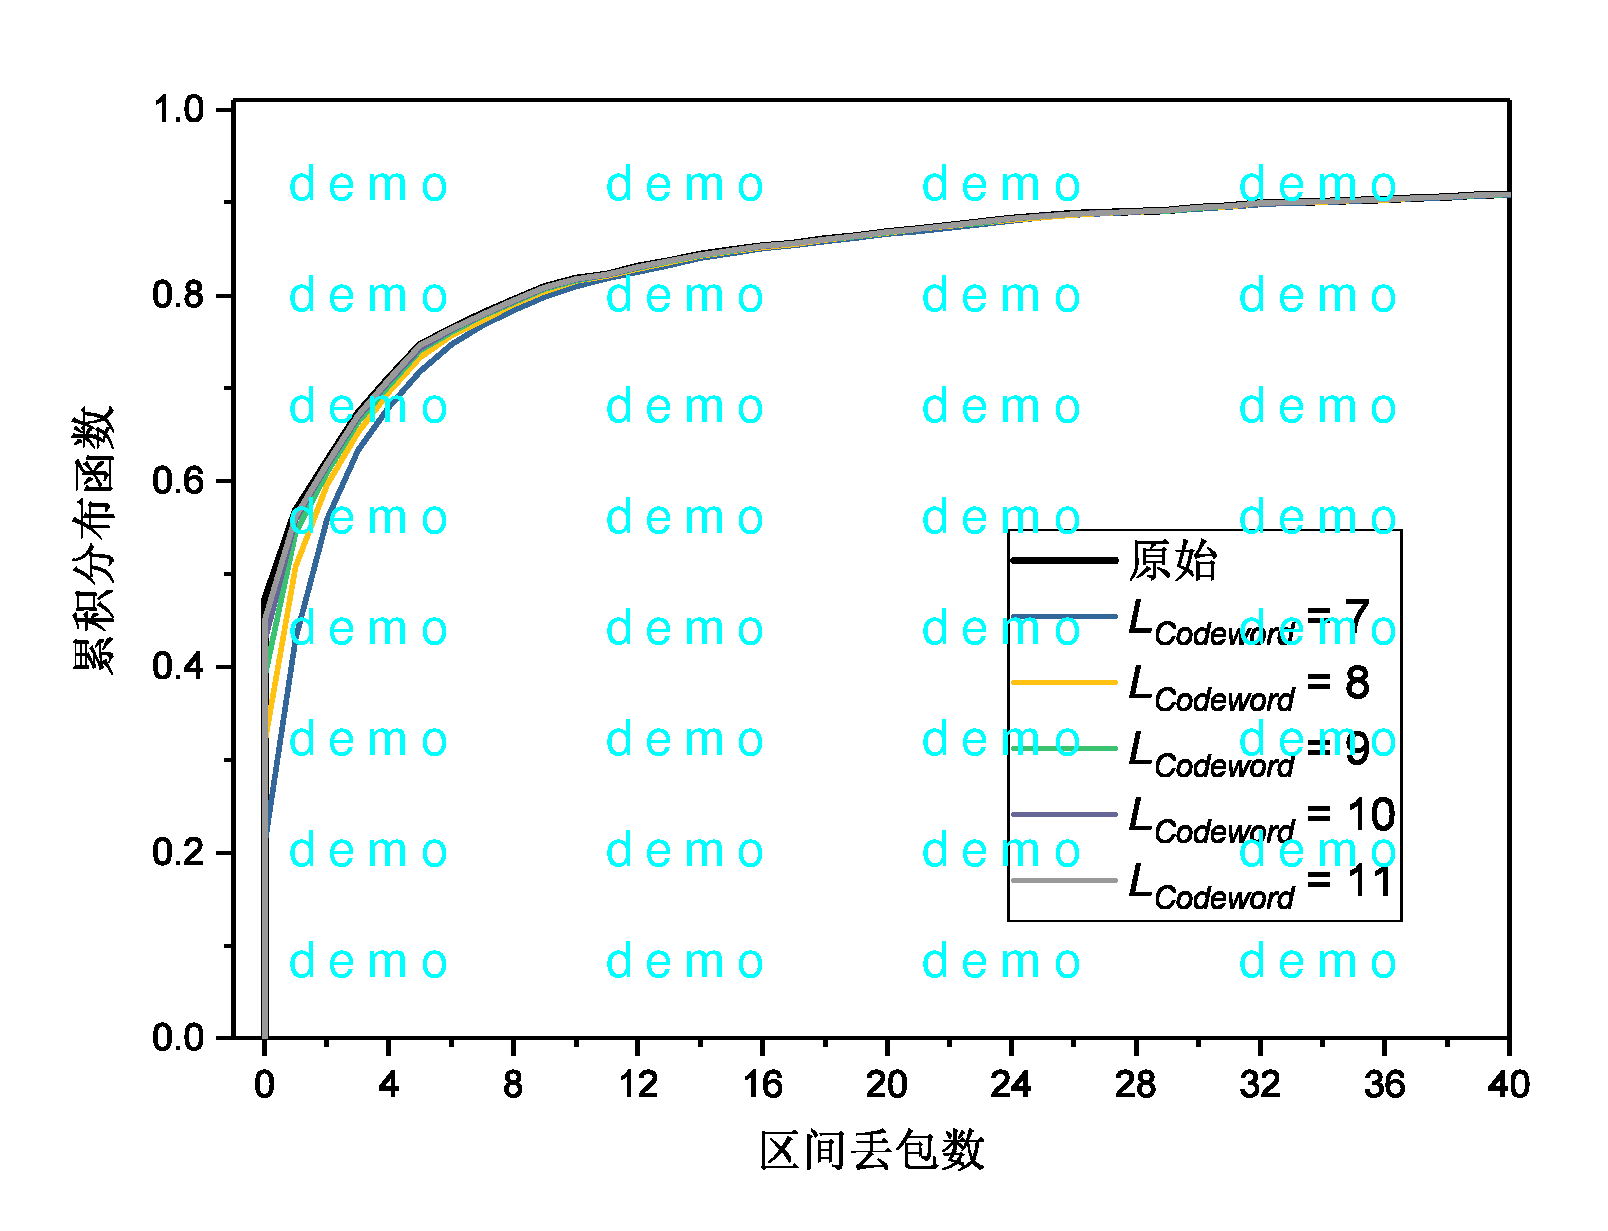
\includegraphics[width=0.48\textwidth]{chapters/chapter5/figures/win100-cdf-good.pdf}
        }
        \subfigure[窗口200时Excellent场景的CDF]{
            \label{fig:5:result:win200:cdf:excellent}
            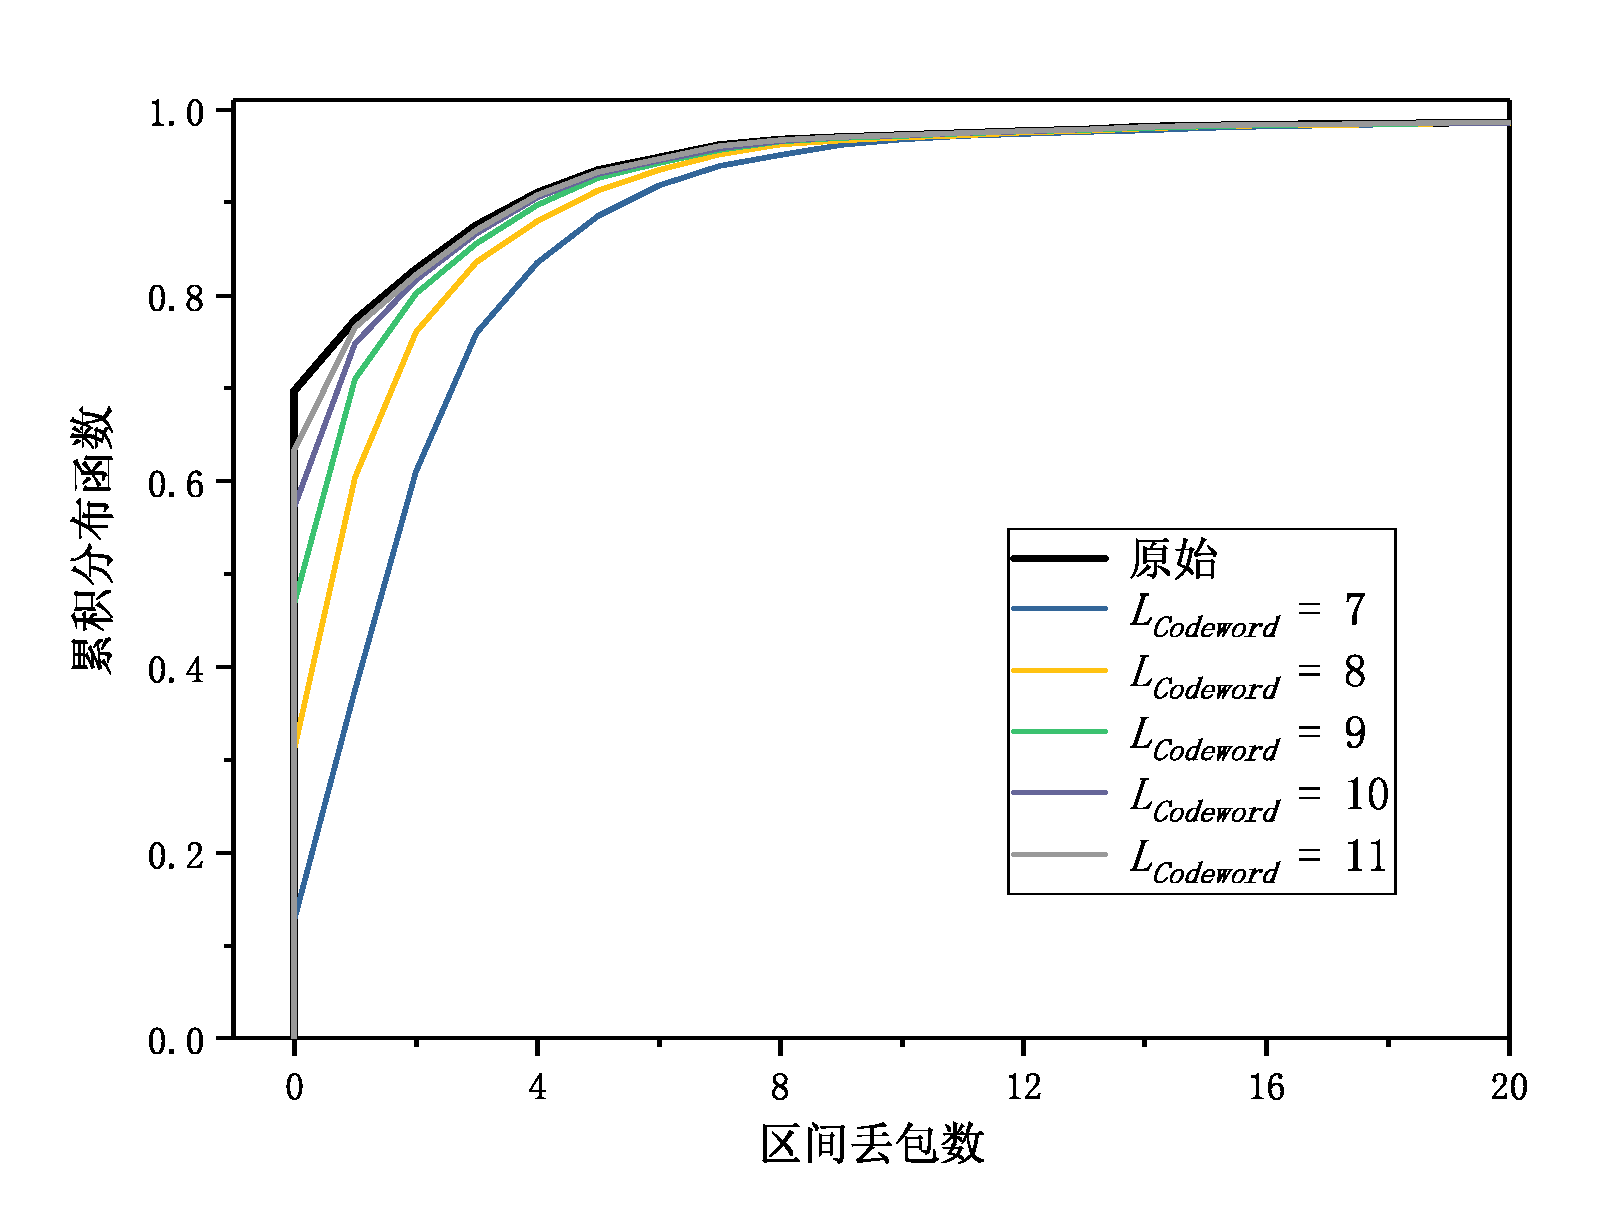
\includegraphics[width=0.48\textwidth]{chapters/chapter5/figures/win200-cdf-excellent.pdf}
        }
        \subfigure[窗口200时Good场景的CDF]{
            \label{fig:5:result:win200:cdf:good}
            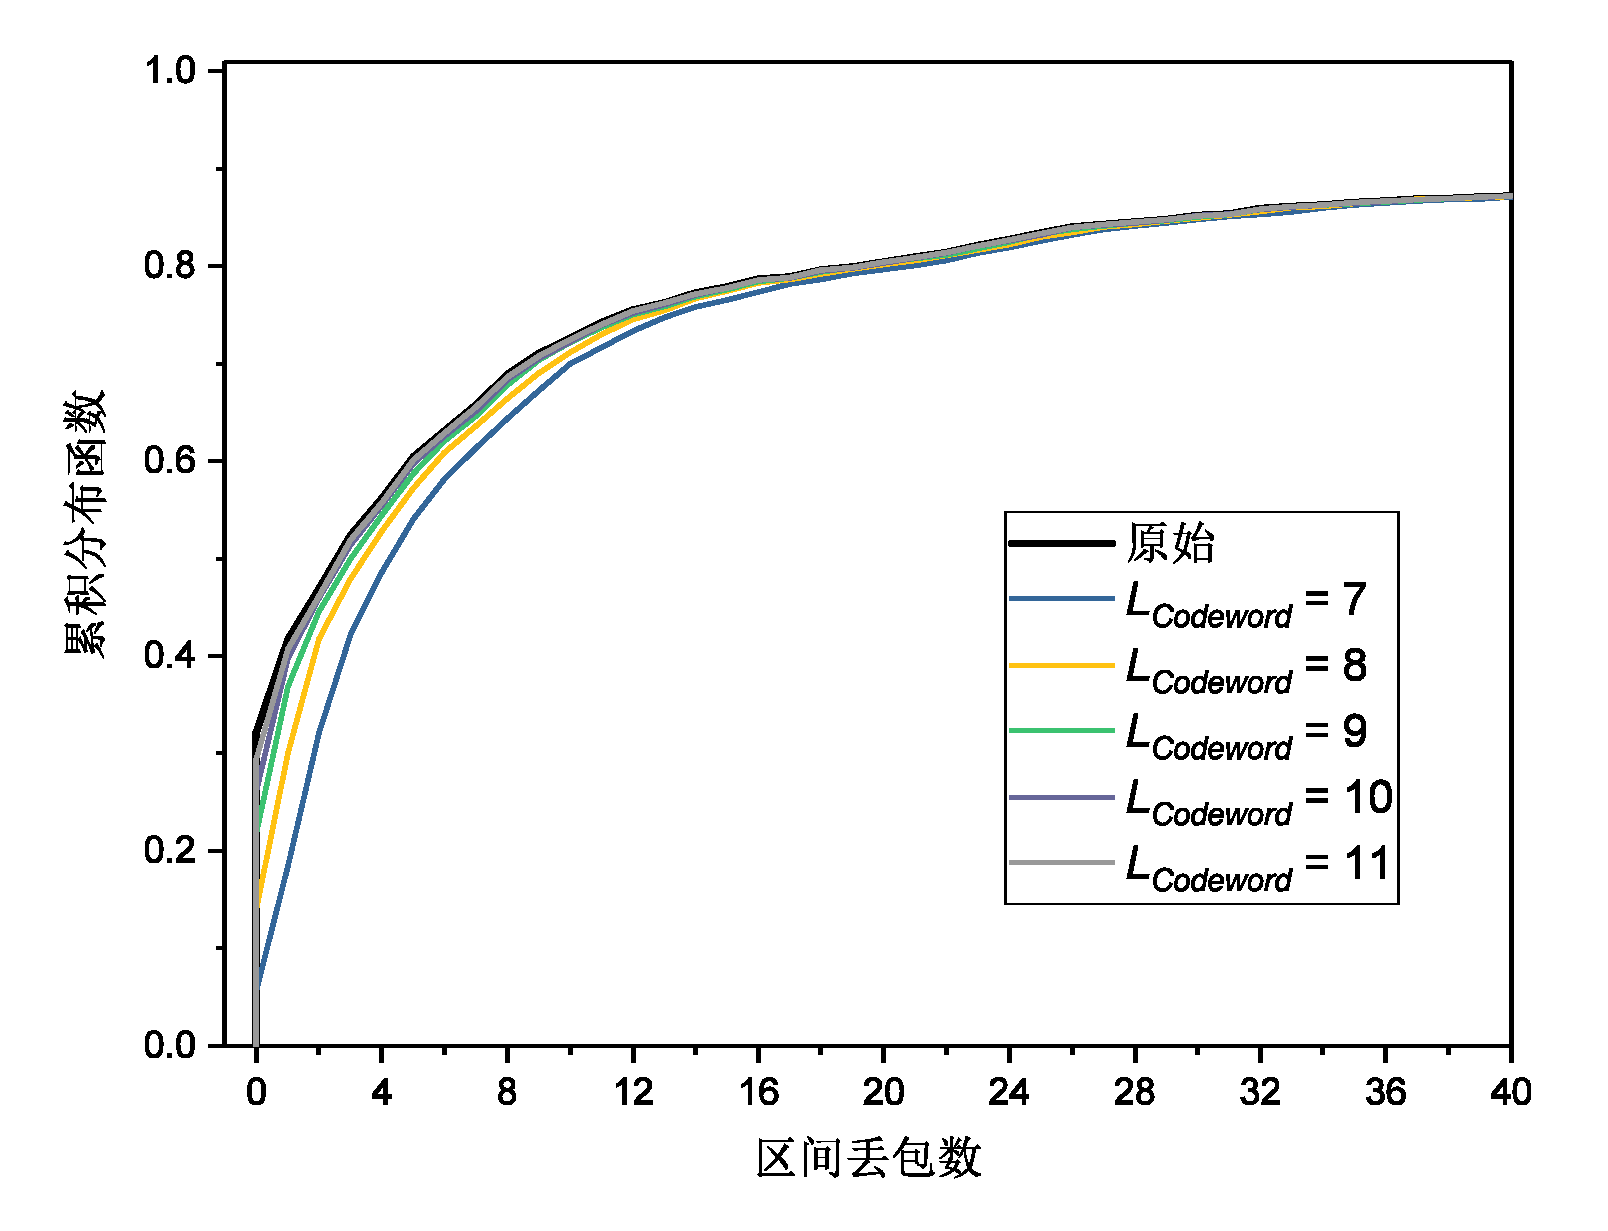
\includegraphics[width=0.48\textwidth]{chapters/chapter5/figures/win200-cdf-good.pdf}
        }
        \caption{区间丢包数的CDF曲线}
        \label{fig:5:result:win:cdf}
    \end{figure}
}

抗检测能力测试,包括对IPD分布、区间丢包数分布、突发丢包长度分布的一致性检测,在检测方法方面使用了CDF曲线检测、分布一致性检测、熵检测及相对距离检测几种不同的检测方式。按照表\nref{tab:3:detect-sum}中的检测方法汇总,汇总不同检测方法的检测结果,得到是否为时间隐通道的判定结论。由于该时间隐通道的丢包密度,主要由参数$L_{Codeword}$决定,因此对抗检测性的评估主要基于不同的$L_{Codeword}$参数配置进行。

\subsubsection{IPD检测}
\label{chap:hash:result:undetectability:ipd}

不同参数下IPD分布的CDF曲线如图\nref{fig:5:result:ipd:cdf},时间隐通道对CDF分布无明显影响,该实验结果与\nref{chap:analyze:result:ipd:cdf}及\nref{chap:zigzag:results:undetectability:ipd}中得到的猜测是结果基本一致。当时间隐通道主动丢包的密度降低,对信道IPD分布的影响减小,通过CDF曲线已经无法检测到明显差异。

\insertTable{
	\begin{table}
      \centering
      \caption{IPD分布检测检出率汇总表}
      \label{tab:5:result:ipd}
          \begin{tabular*}{0.75\textwidth}{@{\extracolsep{\fill}}ccc}
            \toprule
            $L_{Codeword}$ & 方法 & 检出率\\ 
            \midrule
            \multirow{5}{*}{7,\ 8,\ 9,\ 10,\ 11} 
            & K-S检验 & 0\% \\
            & T检验 \& Rank检验 & 0\% \\
            & K-L散度 & 0\% \\
            & Wasserstein距离 & 0\% \\
            & 能量距离 & 0\% \\
            \bottomrule
          \end{tabular*}
    \end{table}
}

IPD分布一致性的量化评估结果如表\nref{tab:5:result:ipd},通过IPD分布情况,无法检测出该时间隐通道。当前时间隐通道的检测方法,多基于IPD分布特征,该时间隐通道的主动丢包比例在1\%以内,因此面对其它检测方法具有足够隐蔽性。

\subsubsection{突发丢包长度检测}
\label{chap:hash:result:undetectability:burst}

突发丢包长度反映了信道中的丢包类型,根据图\nref{fig:3:capture:burst:cdf},在两种场景中的区别主要为连续丢包所占的比例,以及连续丢包的长度。该时间隐通道构建方法,主动丢包造成的是长度为1的离散丢包,造成突发丢包长度分布出现偏离。如图\nref{fig:5:result:burst:cdf},该时间隐通道的主动丢包长度分布对比原始分布,在Excellent场景中导致的偏离更加明显,Good场景下曲线的趋势及取值基本一致。由于Excellent场景中网络噪声强度较弱,平均丢包率小于1\%,因此时间隐通道对分布的影响更加明显;Excellent场景中网络噪声导致的平均丢包率,已经达到了10\%左右,时间隐通道小于1\%的主动丢包率不会导致明显偏离。

\insertTable{
	\begin{table}
      \centering
      \caption{突发丢包长度检测检出率汇总表}
      \label{tab:5:result:burst}
          \begin{tabular*}{0.75\textwidth}{@{\extracolsep{\fill}}cccc}
            \toprule
            场景 & $L_{Codeword}$ & 方法 & 检出率 \\ 
            \midrule
            \multirow{4}{*}{Excellent} 
            & 7,8 & K-L散度 & 100\% \\
            & 9,10,11 & K-L散度 & 0\% \\
            & 7,8,9,10,11 & Wasserstein距离 & 0\% \\
            & 7,8,9,10,11 & 能量距离 & 0\% \\
            \\
            \multirow{3}{*}{Good}
            & 7,8,9,10,11 & K-L散度 & 0\% \\
            & 7,8,9,10,11 & Wasserstein距离 & 0\% \\
            & 7,8,9,10,11 & 能量距离 & 0\% \\
            \bottomrule
          \end{tabular*}
    \end{table}
}

丢突发丢包长度分布的一致性量化检验,结果如表\nref{tab:5:result:burst},其中Good场景下该时间隐通道具有非常好的隐蔽性,在$L_{Codeword}\ge 7$时通过了所有的检测。Excellent场景下,为保证较好的隐蔽性,参数$L_{Codeword}\ge 9$时,在所有的检测方法中才具有隐蔽性。因此,要保证该时间隐通道具备全场景的抗检测能力,参数$L_{Codeword}$应当满足$L_{Codeword}\ge 9$。

\subsubsection{区间丢包数检测}
\label{chap:hash:result:undetectability:plr}

区间丢包数反映了区间内的传输质量,基于主动丢包的时间隐通道,存在固定区间内的丢包行为,通过分析区间丢包数在分布上的差异,判断是否为时间隐通道。两种场景下区间丢包数分布的CDF曲线,如图\nref{fig:5:result:win:cdf},检测中窗口长度设定为100及200。Excellent场景中,如图\nref{fig:5:result:win100:cdf:excellent}及图\nref{fig:5:result:win200:cdf:excellent},时间隐通道的CDF曲线较原始分布已经检测到偏离,并且随着$L_{Codeword}$的减小,相对偏离更加明显。Good场景中,如图\nref{fig:5:result:win100:cdf:good}及图\nref{fig:5:result:win200:cdf:good},时间隐通道的相对偏离减小,该时间隐通道的隐蔽性更好。

\insertTable{
	\begin{table}
      \centering
      \caption{区间丢包数检测检出率汇总表}
      \label{tab:5:result:win}
          \begin{tabular*}{0.75\textwidth}{@{\extracolsep{\fill}}cccc}
            \toprule
            场景 & $L_{Codeword}$ & 方法 & 检出率 \\ 
            \midrule
            \multirow{4}{*}{Excellent} 
            & 7 & Wasserstein距离 & 100\% \\
            & 8,9,10,11 & Wasserstein距离 & 0\% \\
            & 7 & 能量距离 & 100\% \\
            & 8,9,10,11 & 能量距离 & 0\% \\
            \\
            \multirow{6}{*}{Good}
            & 7 & Wasserstein距离 & 100\% \\
            & 8 & Wasserstein距离 & 30\% \\
            & 9,10,11 & Wasserstein距离 & 0\% \\
            & 7 & 能量距离 & 100\% \\
            & 8 & 能量距离 & 30\% \\
            & 9,10,11 & 能量距离 & 0\% \\
            \bottomrule
          \end{tabular*}
    \end{table}
}

在区间丢包数检测方面,该时间隐通道的检出率如表\nref{tab:5:result:win},检出结果与\nref{tab:4:results:win}类似。Excellent场景下,当$L_{Codeword}\ge 8$时,该时间隐通道可以通过区间丢包数的检测;Good场景下,当$L_{Codeword}\ge 9$时,该时间隐通道可以通过区间丢包数的所有检测;Good场景下,当$L_{Codeword}=8$时,该时间隐通道有较高几率通过区间丢包数检测。

\subsubsection{抗检测能力测试汇总}
\label{chap:hash:result:undetectability:sum}

\insertTable{
	\begin{table}
      \centering
      \caption{基于多重校验的时间隐通道检出率汇总表}
      \label{tab:5:result:sum}
          \begin{tabular*}{0.8\textwidth}{@{\extracolsep{\fill}}cccccc}
            \toprule
            \multirow{2}{*}{场景} 
            & \multicolumn{5}{c}{$L_{Codeword}$} \\
            & 7 & 8 & 9 & 10 & 11 \\
            \midrule
            Excellent & 100\% & 100\% & 0\% & 0\% & 0\% \\
            Good & 100\% & 30\% & 0\% & 0\% & 0\% \\
            \bottomrule
          \end{tabular*}
    \end{table}
}

根据表\nref{tab:3:detect-sum}中的所有检测项,该时间隐通道的总体检出率结果如表\nref{tab:5:result:sum}。Good场景中,该事件隐通道构建方法具有较好的隐蔽性,在$L_{Codeword}=8$时仍有几率通过检测。为通过所有场景下的所有测试,该时间隐通道的传输参数$L_{Codeword}$,应当满足$L_{Codeword}\ge 9$。

\subsection{鲁棒性测试}
\label{chap:hash:result:robustness}

鲁棒性测试的评估指标是误码率,计算方法如公式(\nref{equ:2:ber})。该时间隐通道中,影响误码率的传输参数包括$L_{Codeword}$、$L_{HASH}$、$L_{CRC}$、$R$及$M_{cols}$,因此鲁棒性评估过程主要围绕这些参数进行。在测试环境方面,除了真实的Excellent场景及Good场景,设置了4种不同比例的随机丢包场景。

\insertFigure{
	\begin{figure}
        \centering
        \subfigure[Excellent场景的平均误码率]{
            \label{fig:5:result:ber:mcols:excellent}
            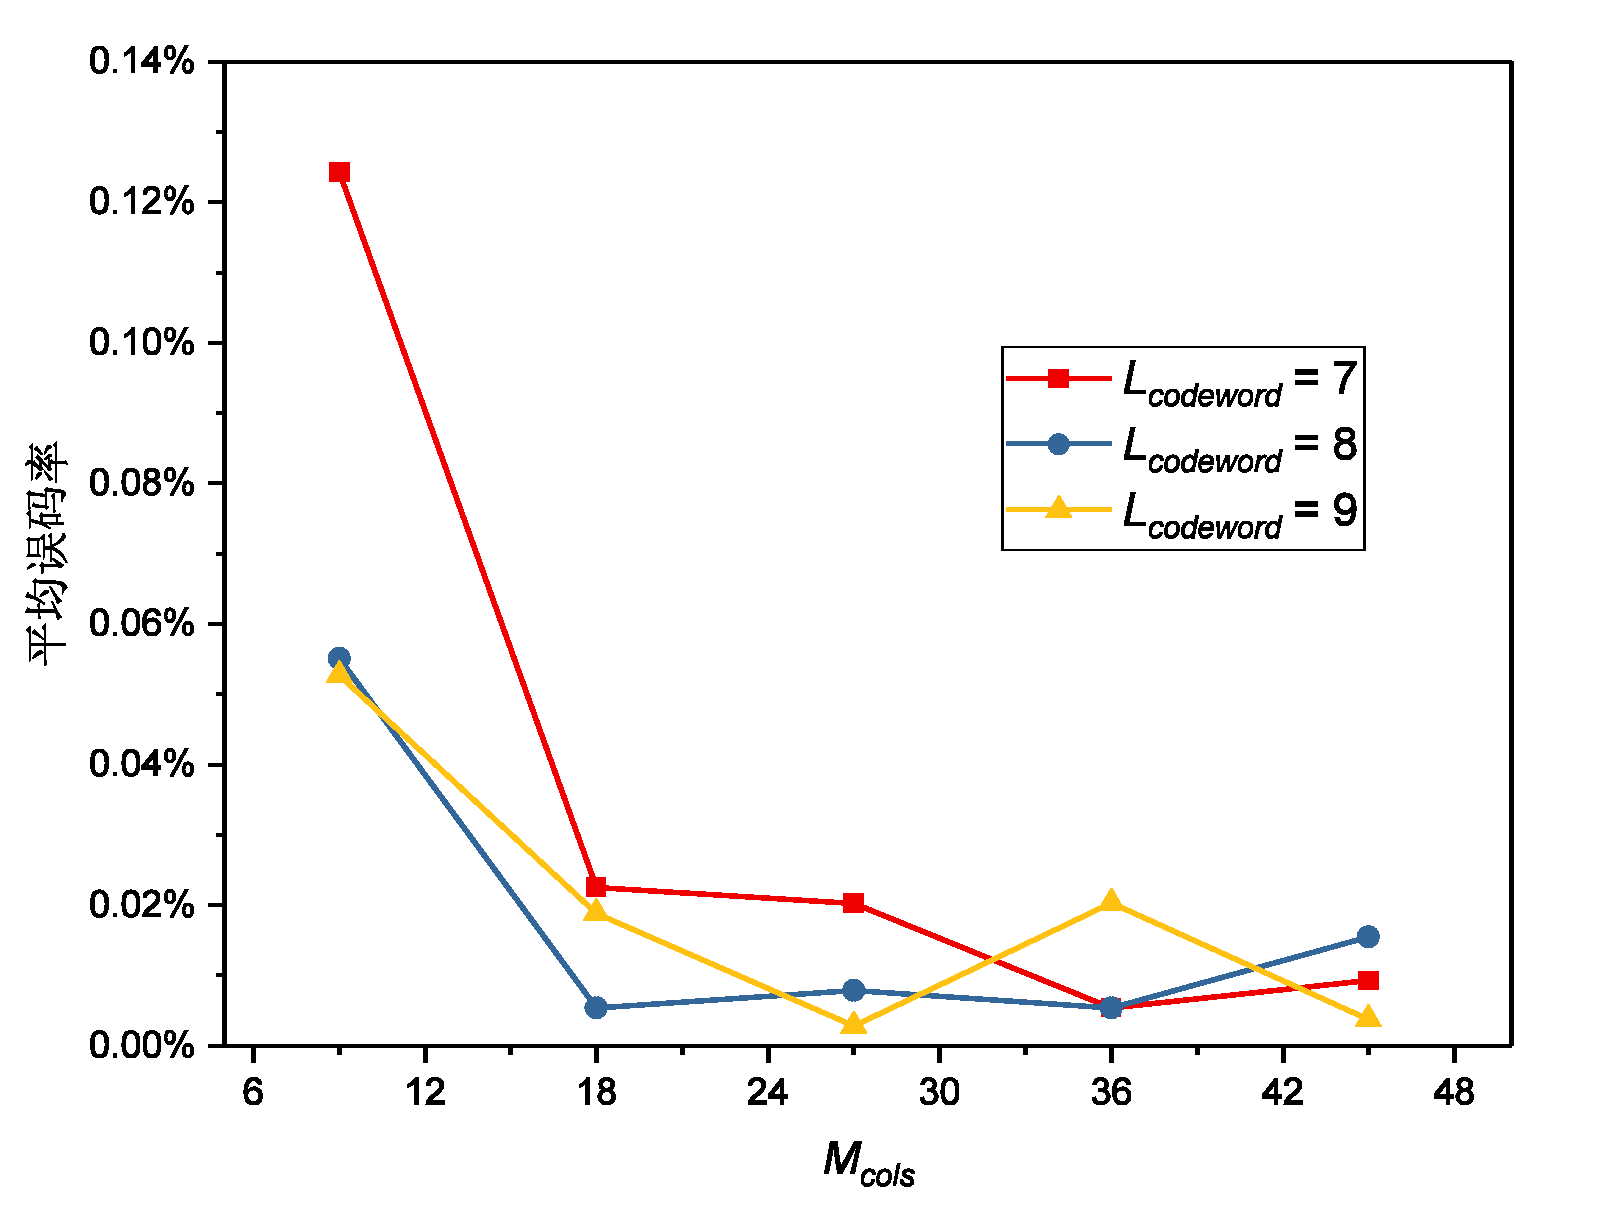
\includegraphics[width=0.48\textwidth]{chapters/chapter5/figures/ber-mcols-excellent.pdf}
        }
        \subfigure[Good场景的平均误码率]{
            \label{fig:5:result:ber:mcols:good}
            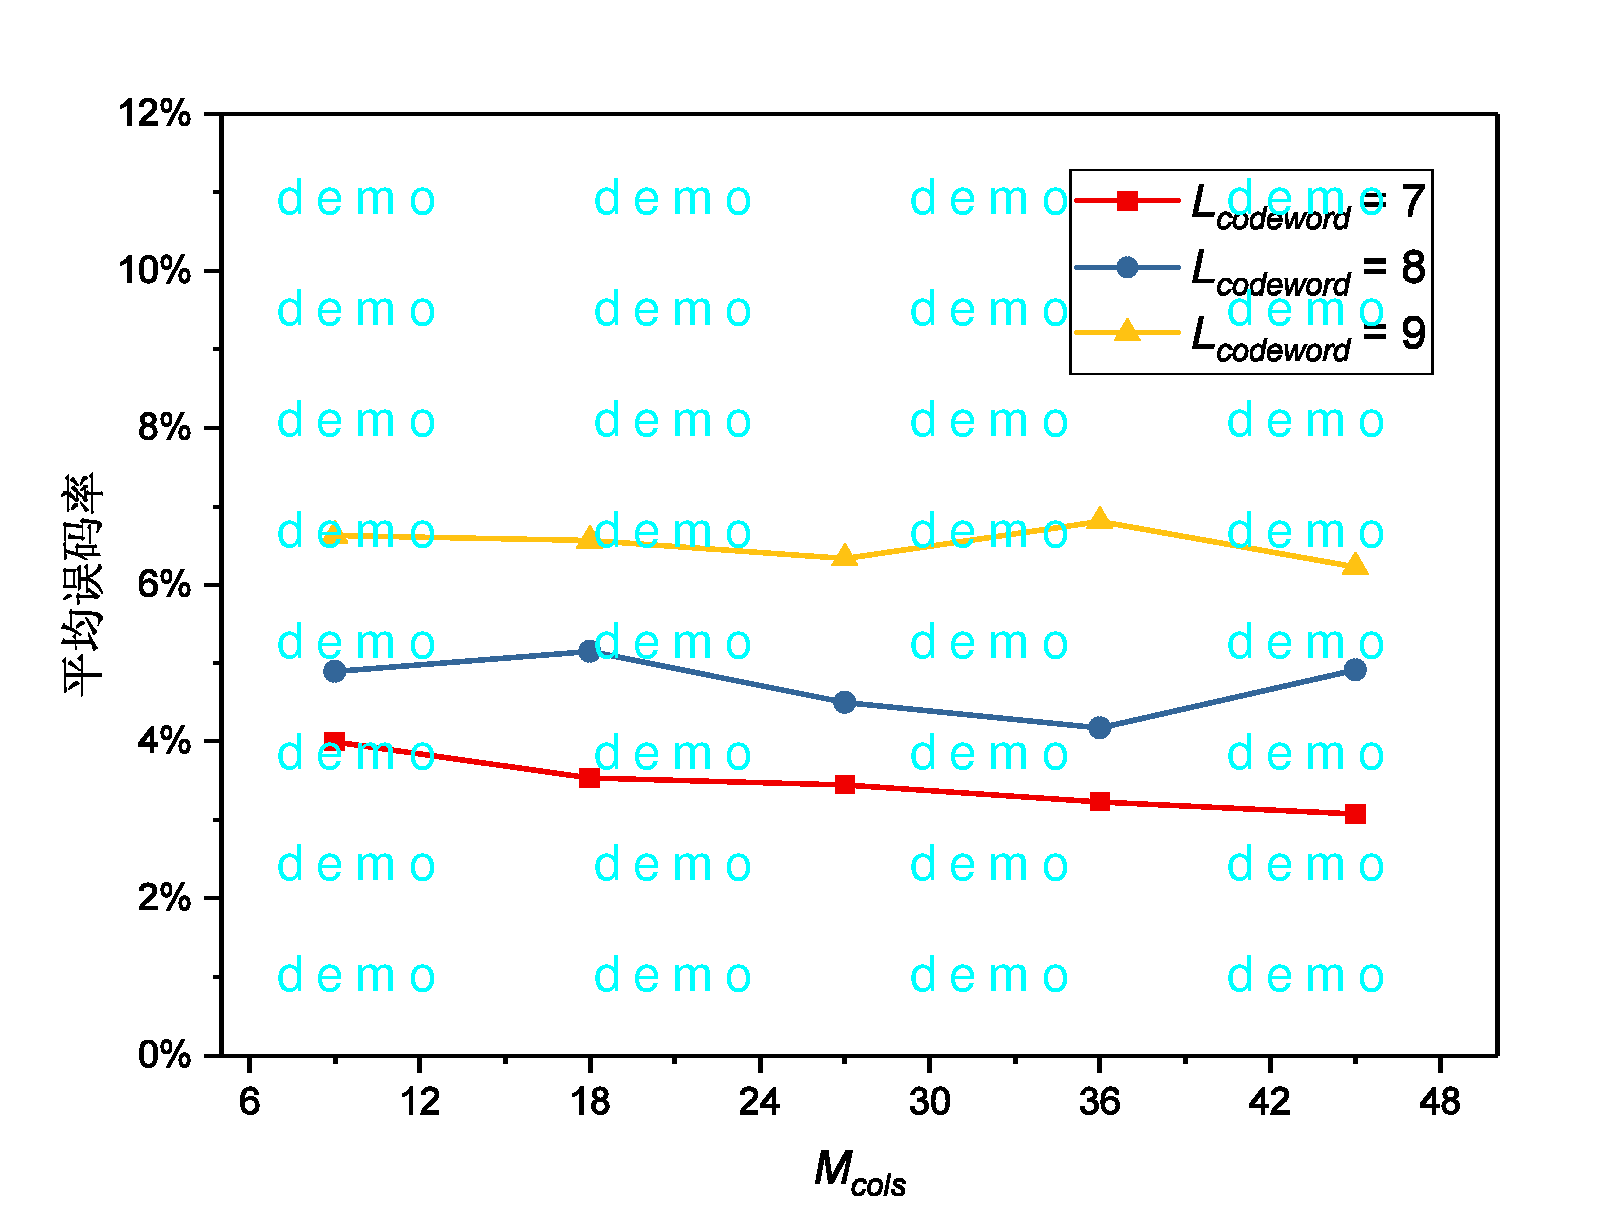
\includegraphics[width=0.48\textwidth]{chapters/chapter5/figures/ber-mcols-good.pdf}
        }
        \caption{平均误码率与$M_{cols}$的折线图}
        \label{fig:5:result:ber:mcols}
    \end{figure}

    \begin{figure}
        \centering
        \subfigure[Excellent场景的平均误码率]{
            \label{fig:5:result:ber:lcodeword:excellent}
            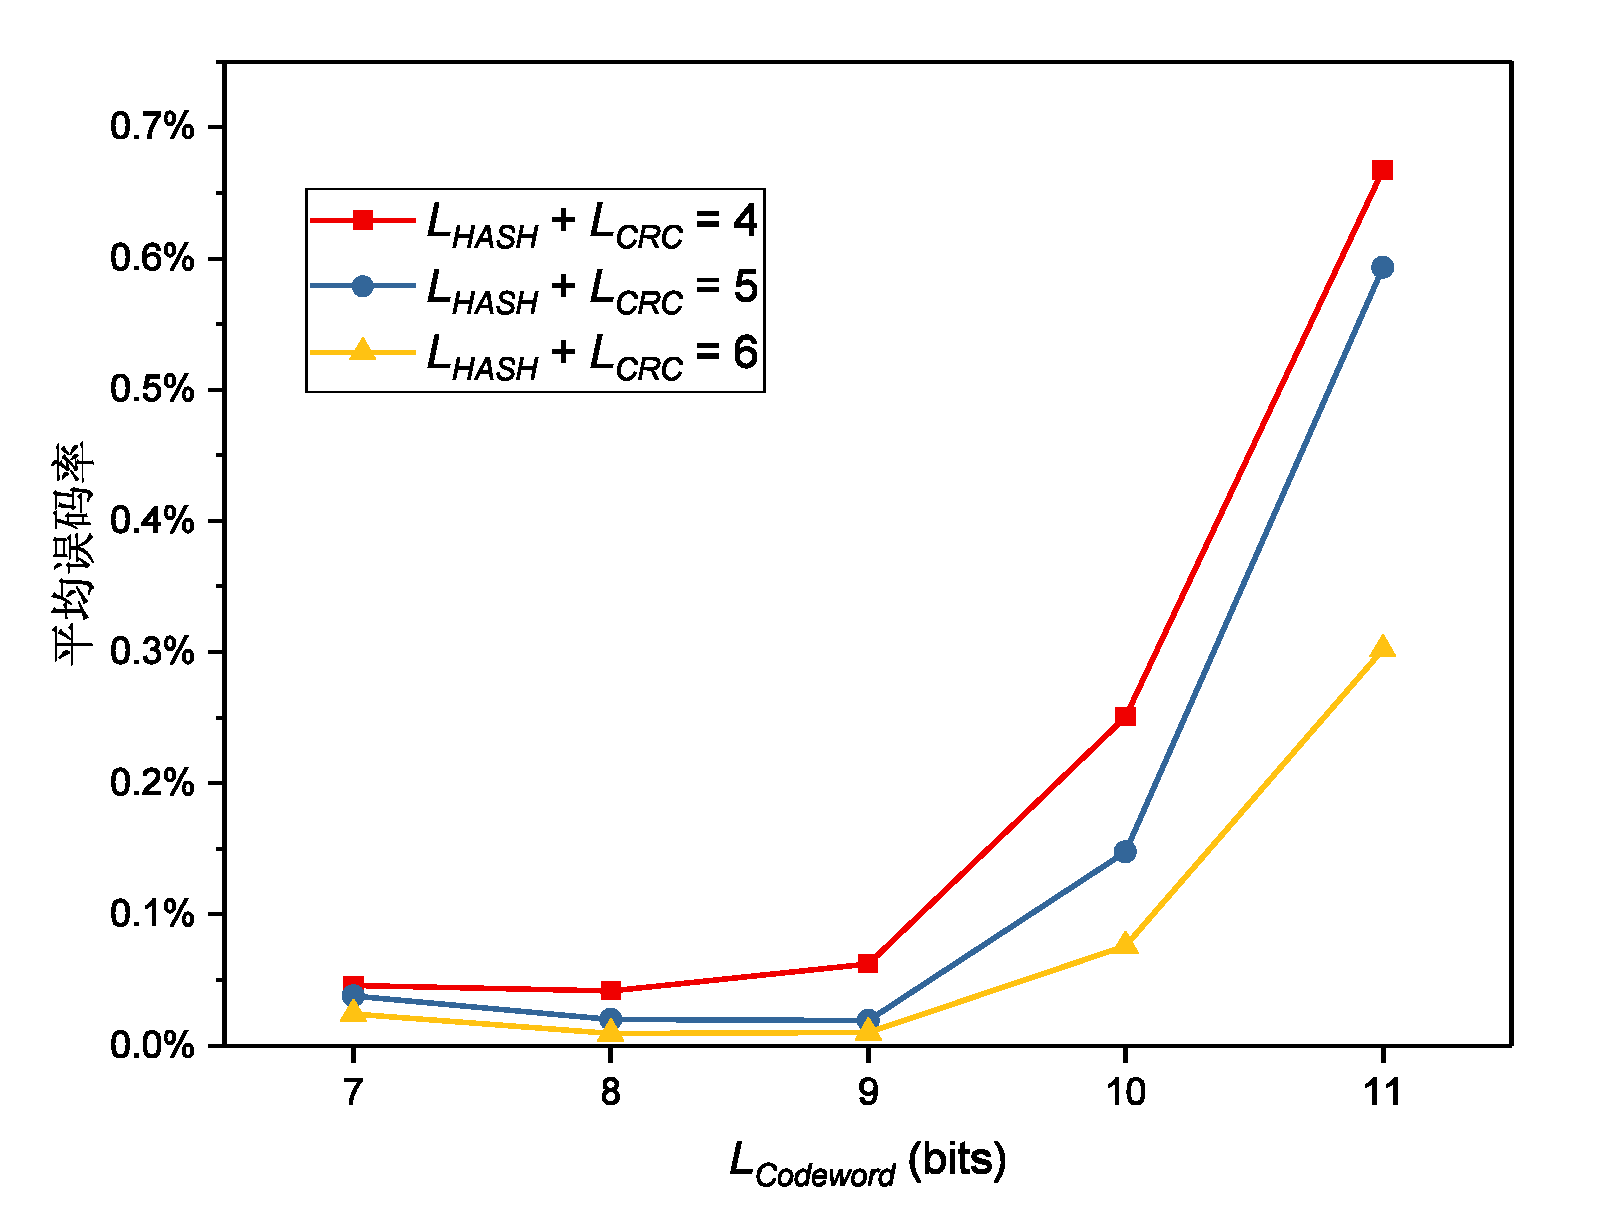
\includegraphics[width=0.48\textwidth]{chapters/chapter5/figures/ber-lcodeword-excellent.pdf}
        }
        \subfigure[Good场景的平均误码率]{
            \label{fig:5:result:ber:lcodeword:good}
            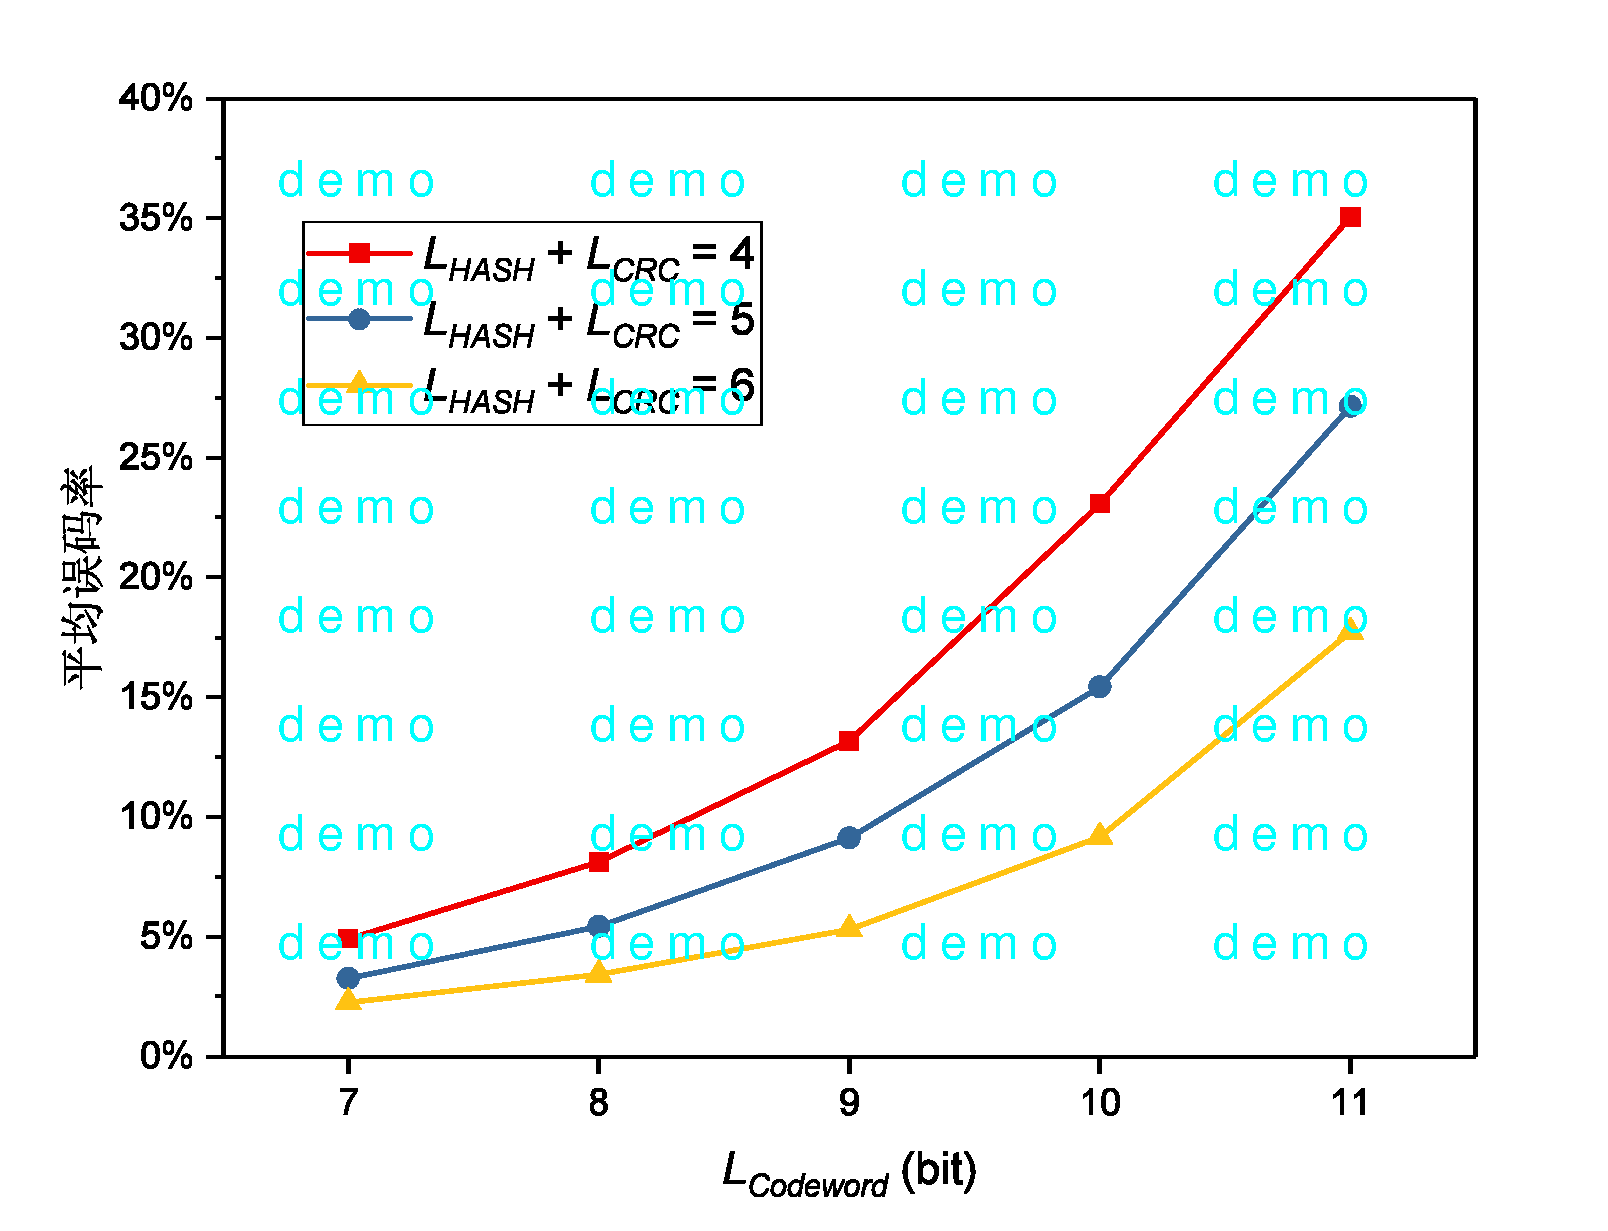
\includegraphics[width=0.48\textwidth]{chapters/chapter5/figures/ber-lcodeword-good.pdf}
        }
        \caption{平均误码率与$L_{Codeword}$的折线图}
        \label{fig:5:result:ber:lcodeword}
    \end{figure}

    \begin{figure}
        \centering
        \subfigure[Excellent场景的平均误码率]{
            \label{fig:5:result:ber:lhash:excellent}
            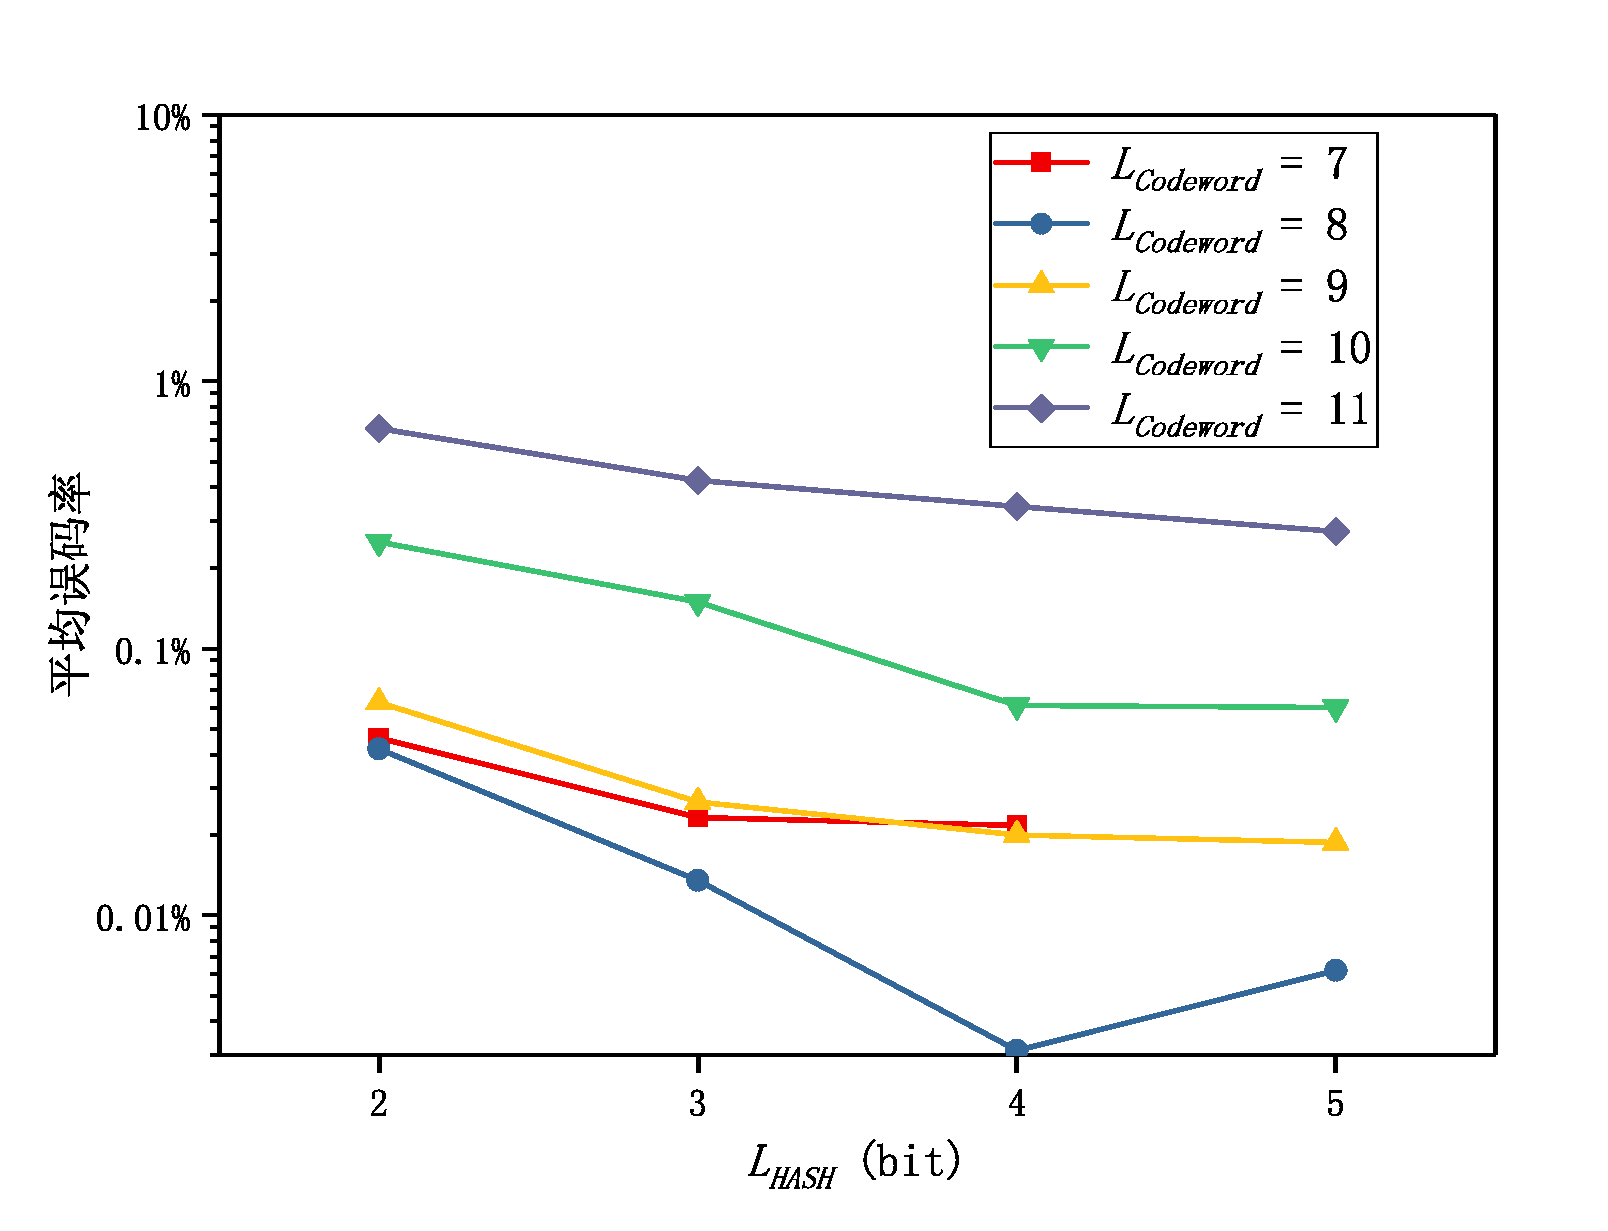
\includegraphics[width=0.48\textwidth]{chapters/chapter5/figures/ber-lhash-excellent.pdf}
        }
        \subfigure[Good场景的平均误码率]{
            \label{fig:5:result:ber:lhash:good}
            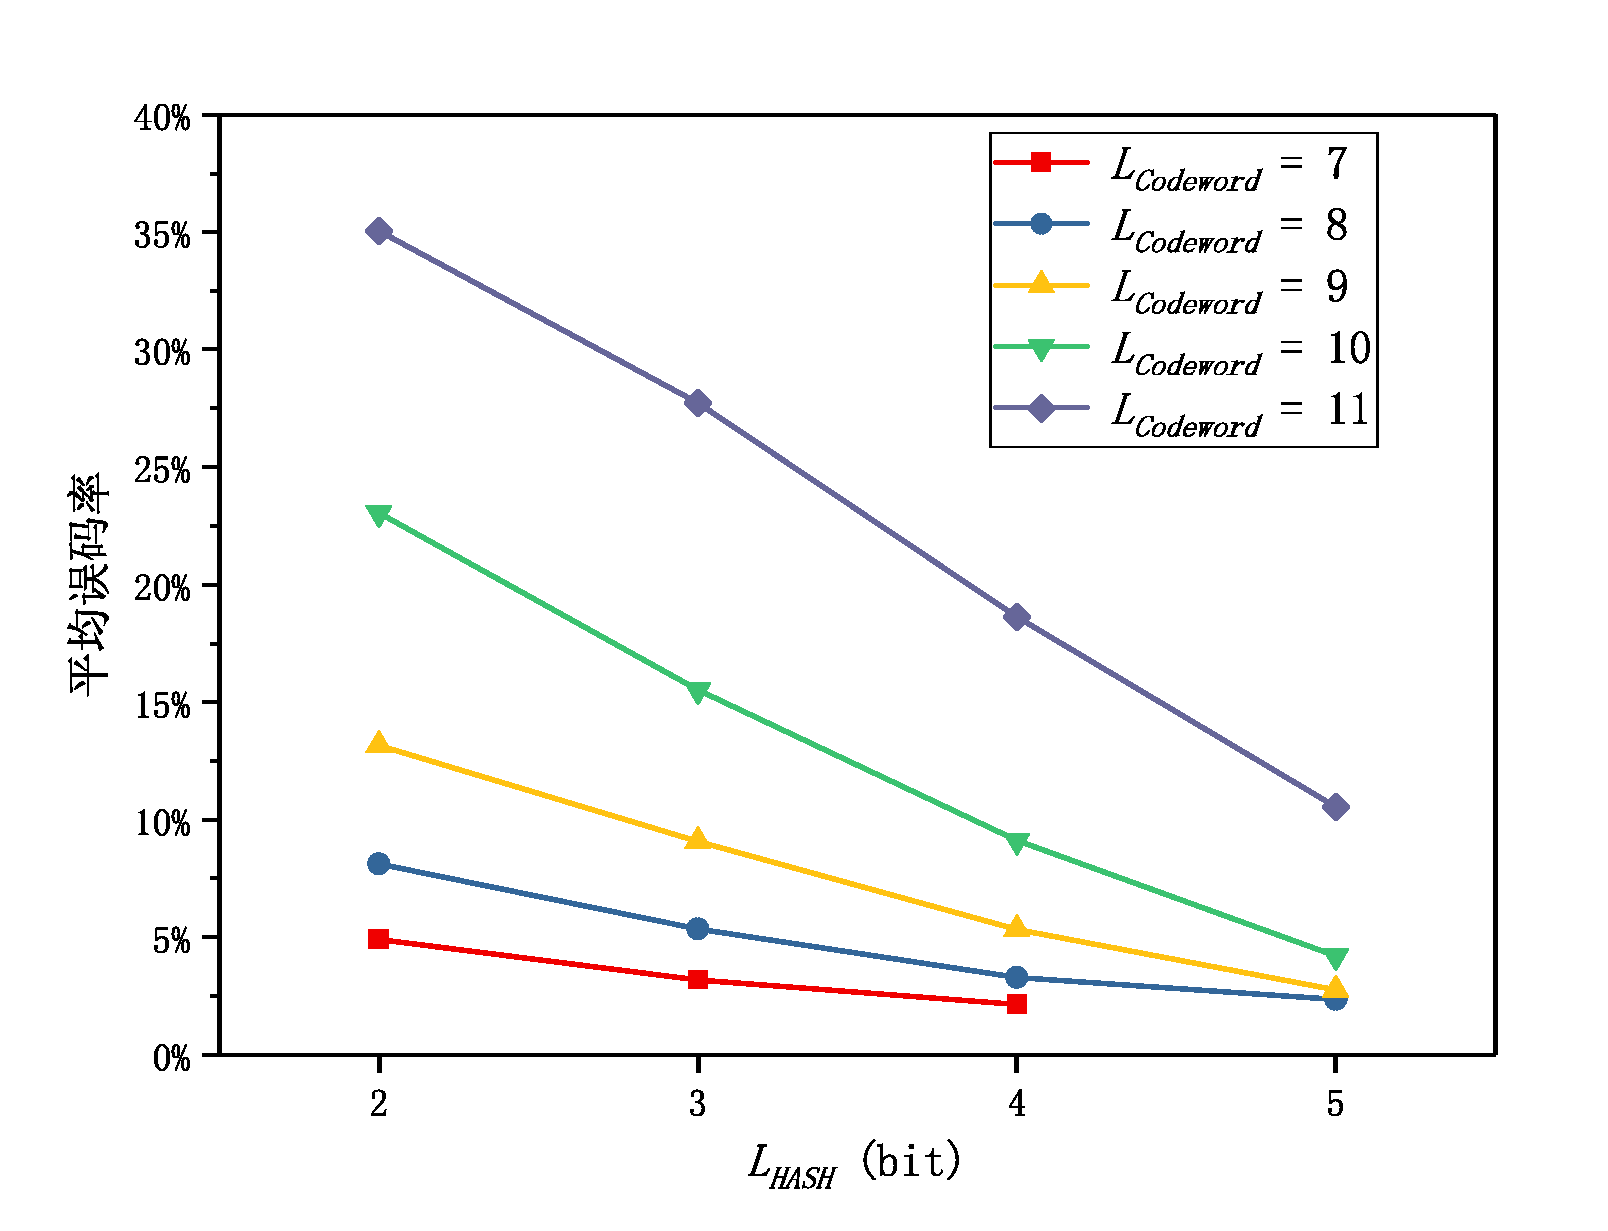
\includegraphics[width=0.48\textwidth]{chapters/chapter5/figures/ber-lhash-good.pdf}
        }
        \caption{平均误码率与$L_{HASH}$的折线图}
        \label{fig:5:result:ber:lhash}
    \end{figure}

    \begin{figure}
        \centering
        \subfigure[Excellent场景的平均误码率]{
            \label{fig:5:result:ber:lcrc:excellent}
            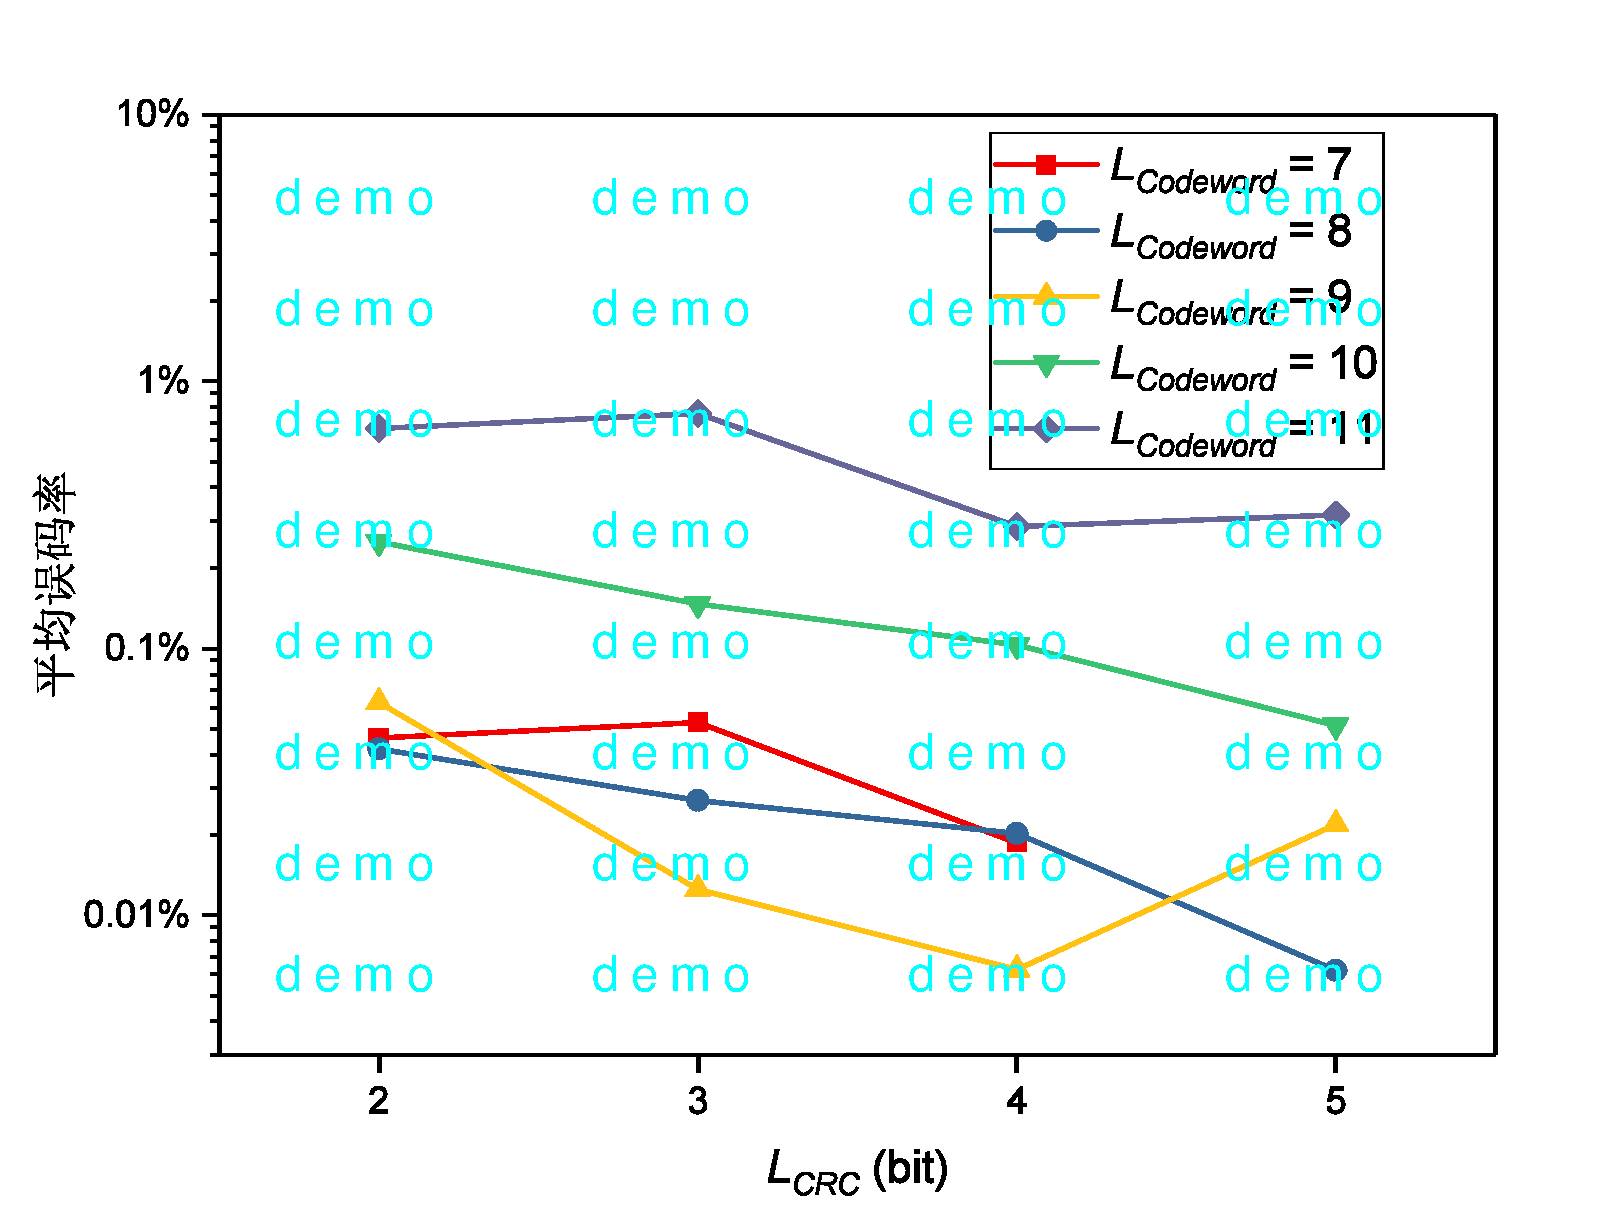
\includegraphics[width=0.48\textwidth]{chapters/chapter5/figures/ber-lcrc-excellent.pdf}
        }
        \subfigure[Good场景的平均误码率]{
            \label{fig:5:result:ber:lcrc:good}
            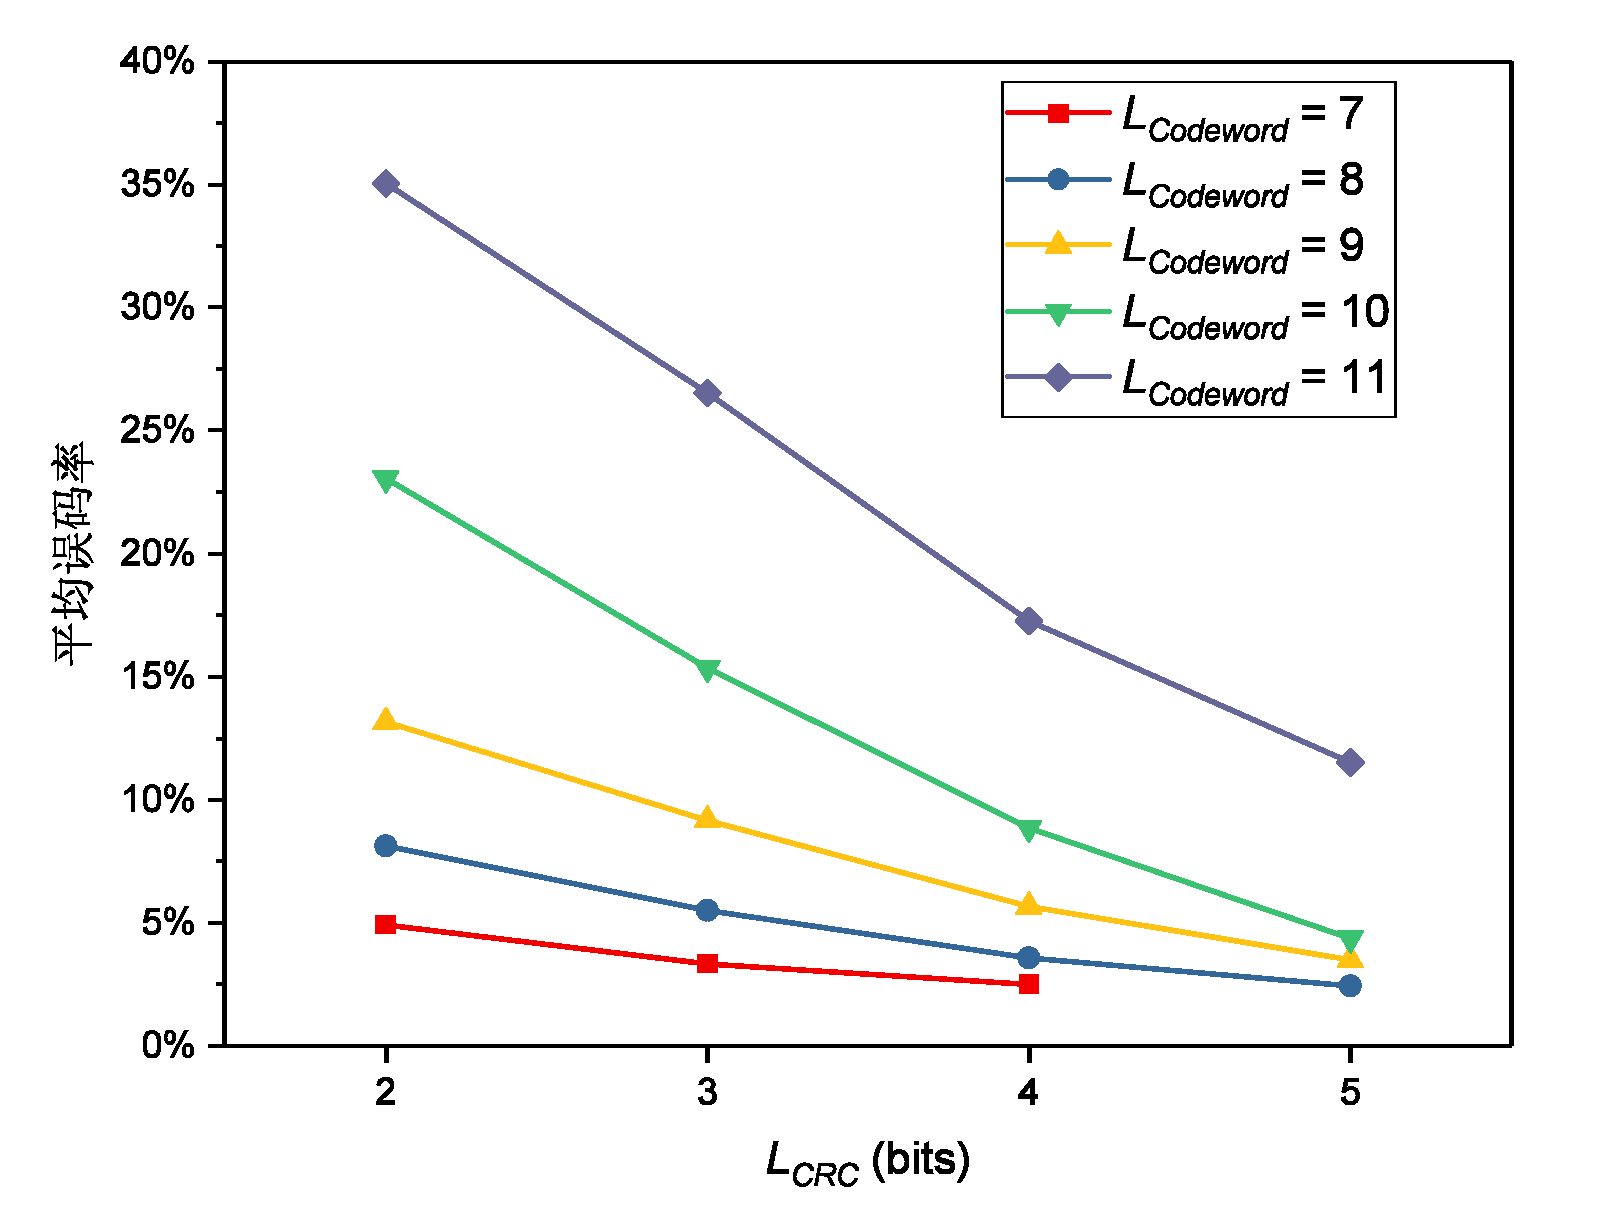
\includegraphics[width=0.48\textwidth]{chapters/chapter5/figures/ber-lcrc-good.pdf}
        }
        \caption{平均误码率与$L_{CRC}$的折线图}
        \label{fig:5:result:ber:lcrc}
    \end{figure}

    \begin{figure}
        \centering
        \subfigure[Excellent场景的平均误码率]{
            \label{fig:5:result:ber:r:excellent}
            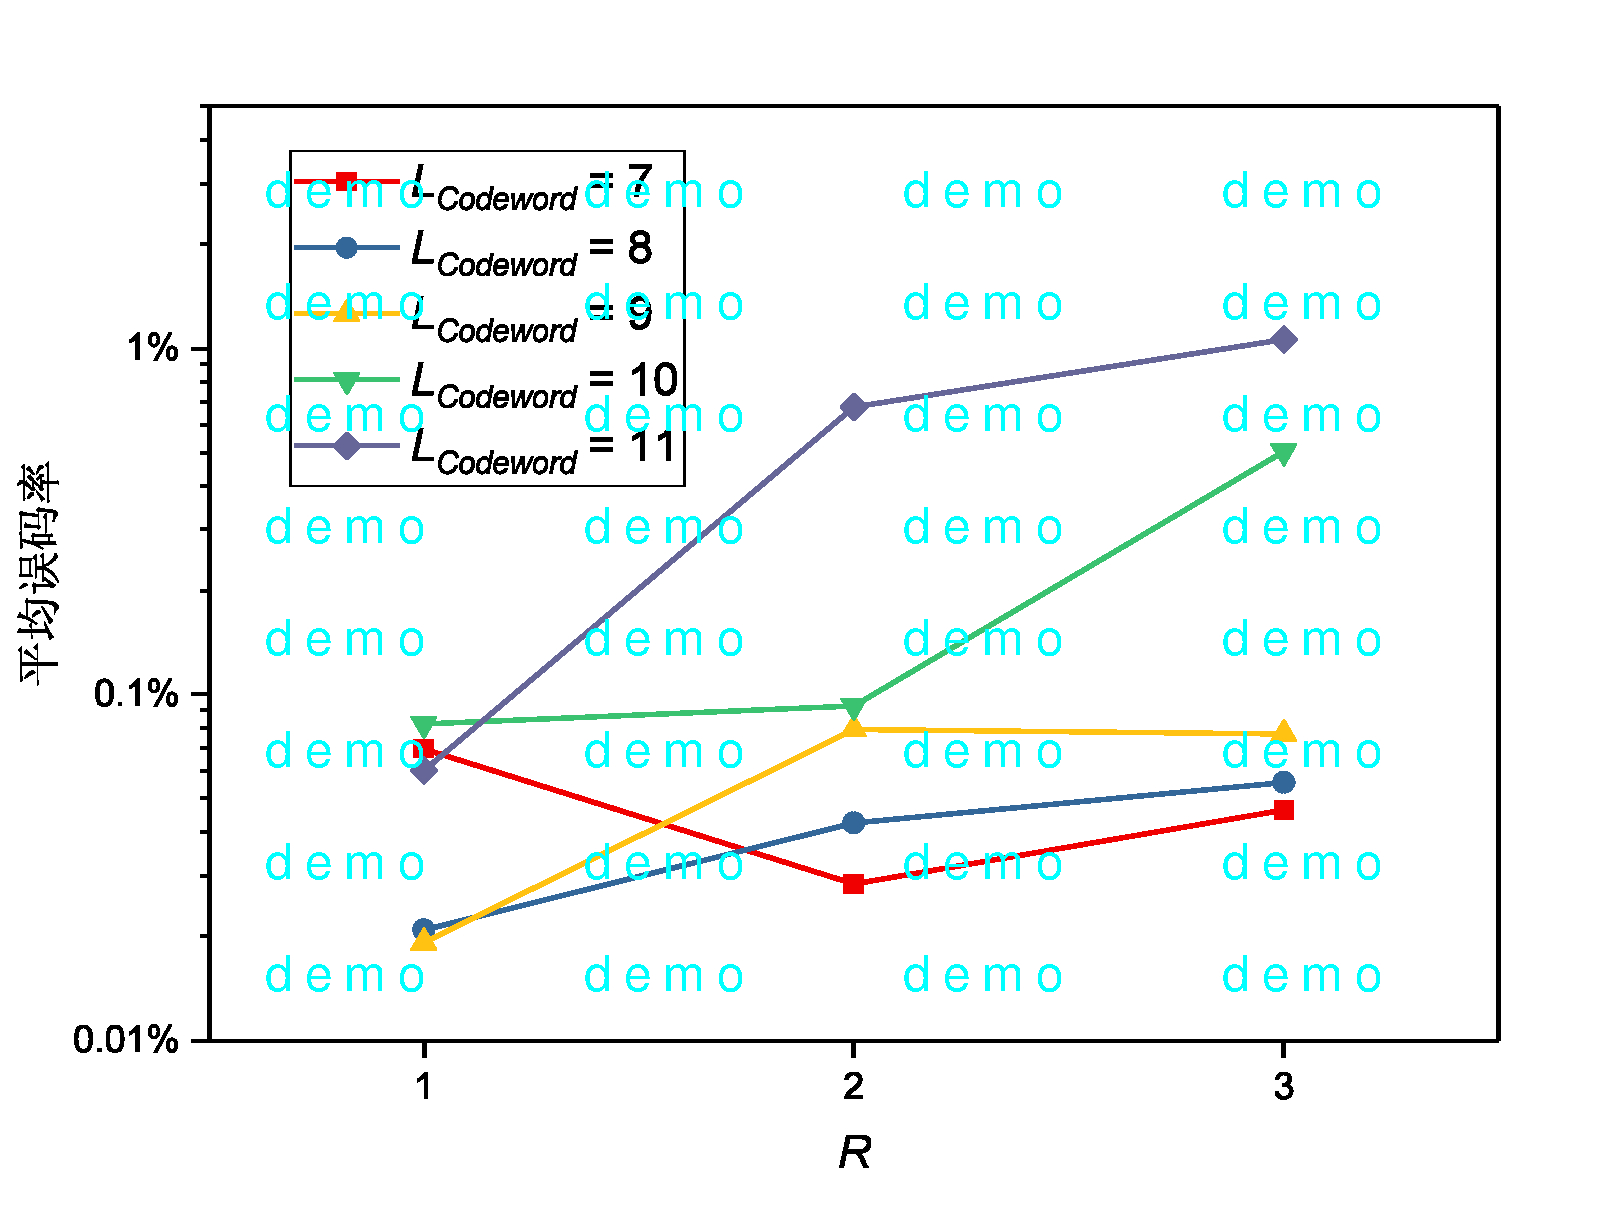
\includegraphics[width=0.48\textwidth]{chapters/chapter5/figures/ber-r-excellent.pdf}
        }
        \subfigure[Good场景的平均误码率]{
            \label{fig:5:result:ber:r:good}
            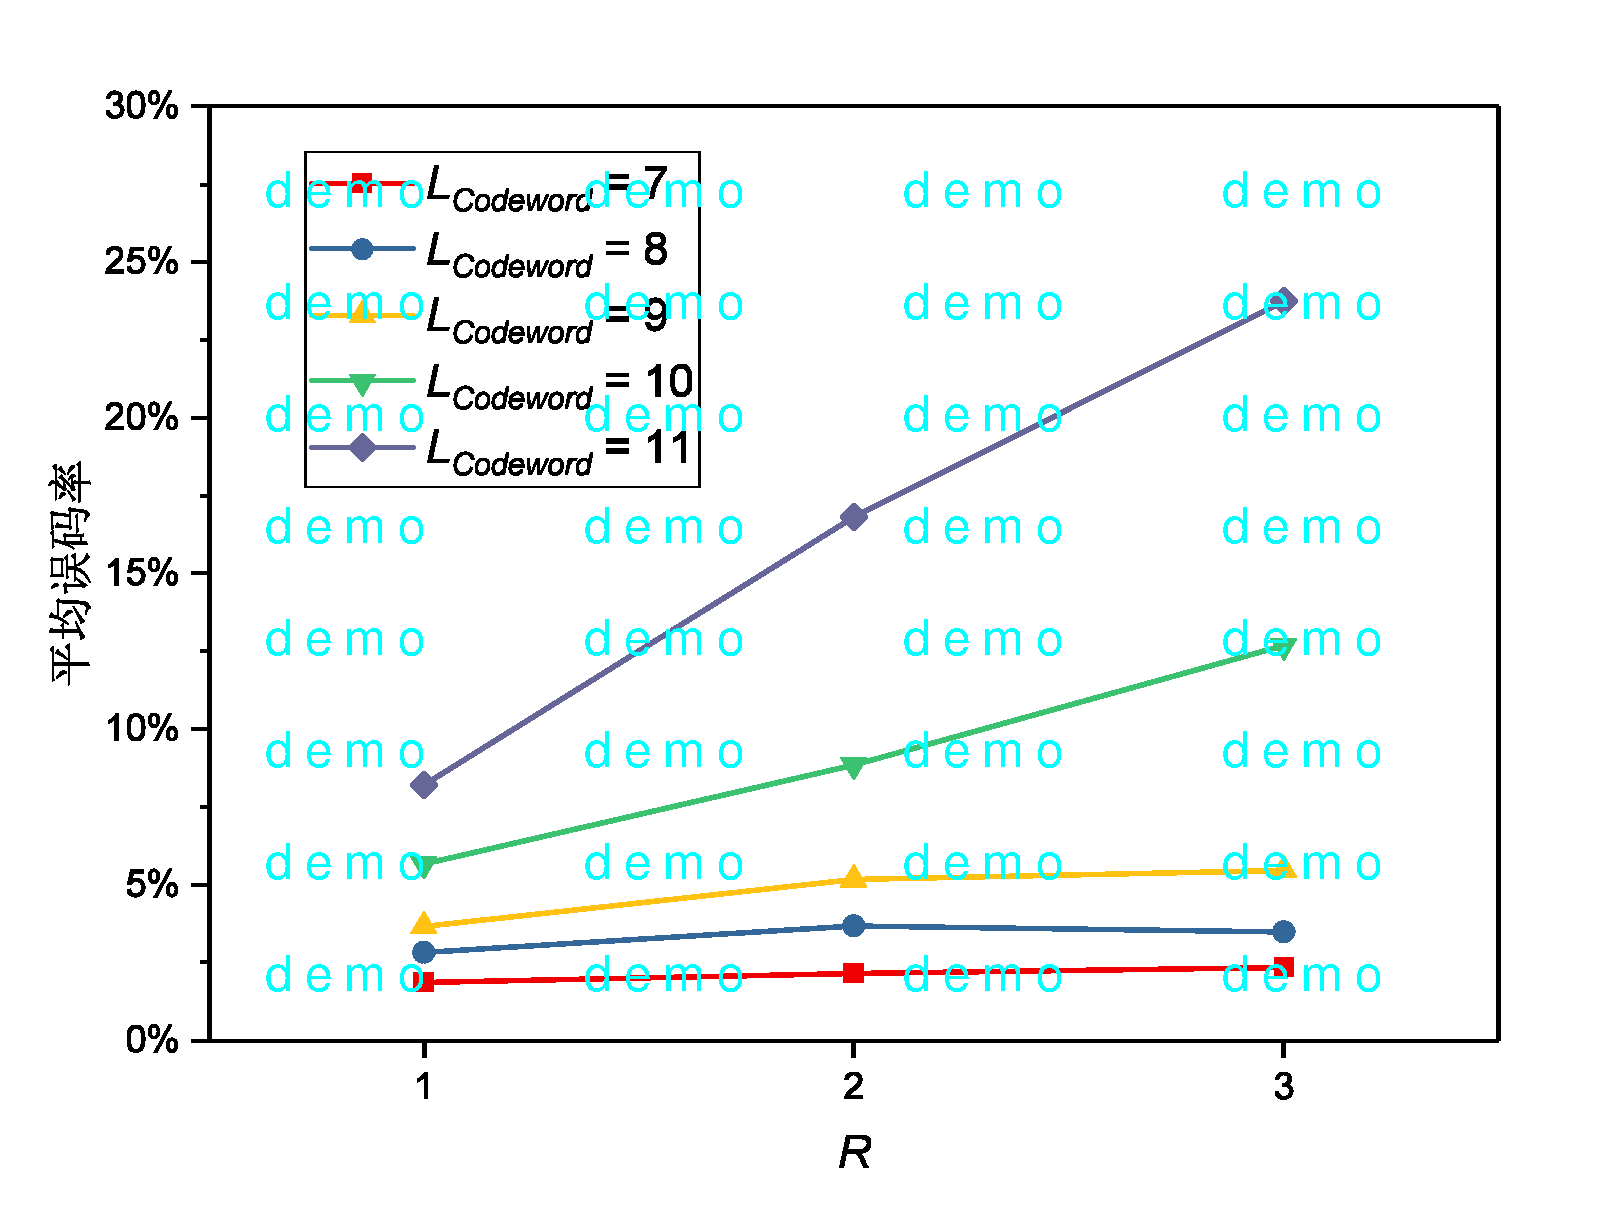
\includegraphics[width=0.48\textwidth]{chapters/chapter5/figures/ber-r-good.pdf}
        }
        \caption{平均误码率与$R$的折线图}
        \label{fig:5:result:ber:r}
    \end{figure}
}

Excellent场景及Good场景下的平均误码率水平,如图\nref{fig:5:result:ber:mcols}、图\nref{fig:5:result:ber:lcodeword}、图\nref{fig:5:result:ber:lhash}、图\nref{fig:5:result:ber:lcrc}及图\nref{fig:5:result:ber:r}。其中,图\nref{fig:5:result:ber:mcols}为平均误码率与参数$M_{cols}$的关系。图\nref{fig:5:result:ber:mcols:excellent}中,Excellent场景下误码率水平已经较低,通过增大$M_{cols}$能够在一定程度上降低平均误码率,但在不增加校验强度的情况下作用有限。图\nref{fig:5:result:ber:mcols:good}中,Good场景下误码率水平较高,通过增大$M_{cols}$能够在一定程度上降低误码率,但作用效果有限。

图\nref{fig:5:result:ber:lcodeword}中,在两种场景下,维持$L_{HASH}+L—_{CRC}$不变的情况下,增大$L_{Codeword}$会导致误码率显著增加。由于$L_{Codeword}$ bit数据对应的数据包数量为$2^{L_{Codeword}}$,$L_{Codeword}$每增加1 bit,数据包数量就要翻倍,相同丢包率下每组的噪声强度也响应加倍,平均误码率也会随之升高。因此,该时间隐通道要获取较好的鲁棒性,参数$L_{Codeword}$要尽可能降低。

图\nref{fig:5:result:ber:lhash}中,两种场景下平均误码率随着$L_{HASH}$增大而减小,并且在Good场景中平均误码率下降更加明显。类似的,图\nref{fig:5:result:ber:lcrc}中,两种场景下的平均误码率随着$L_{CRC}$增大而减小。在Excellent场景中,平均误码率已经处于较低水平,因此增大$L_{HASH}$及$L_{CRC}$产生的效果有限;而在Good场景中,随着$L_{HASH}+L_{CRC}$总位数的增加,平均误码率下降较快。特别的,一定程度上增大$L_{Codeword}$,可以在码字中嵌入更多的校验位数,因此在改善鲁棒性方面存在一定的积极意义。

图\nref{fig:5:result:ber:r}中,随着参数$R$的增大,两种场景下的平均误码率出现显著增长。由于$R$决定了基于HASH的码字间校验的复位周期,$R$越大则复位周期越长,噪声在解调过程中的累积效应越明显,出现匹配错误的概率增大,鲁棒性下降。同时,即使在Good场景中,在一定的参数配置下,增大$R$周期长度,可以在维持鲁棒性的前提下,保证一定的传输性能。

\insertFigure{
	\begin{figure}
        \centering
        \subfigure[$L_{Codeword}$与平均误码率]{
            \label{fig:5:result:ber:random:lcodeword}
            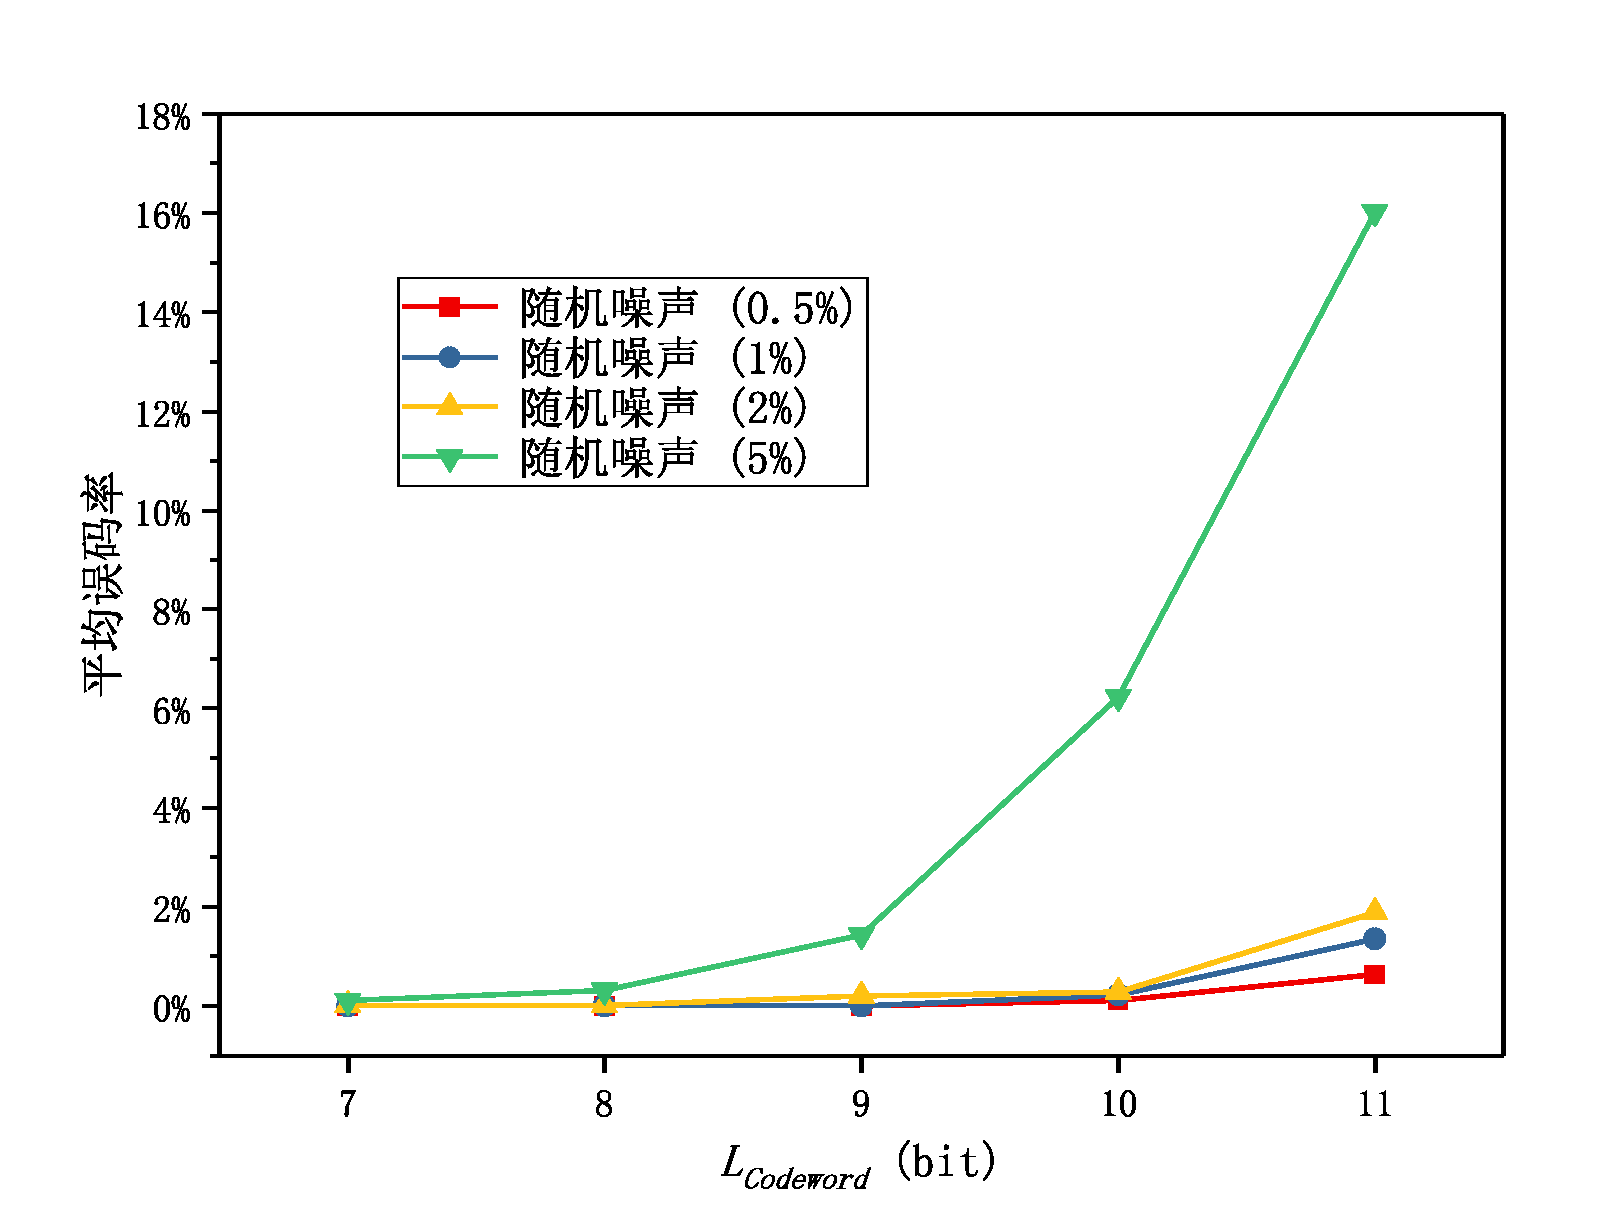
\includegraphics[width=0.48\textwidth]{chapters/chapter5/figures/ber-lcodeword-random.pdf}
        }
        \subfigure[$L_{HASH}$与平均误码率]{
            \label{fig:5:result:ber:random:lhash}
            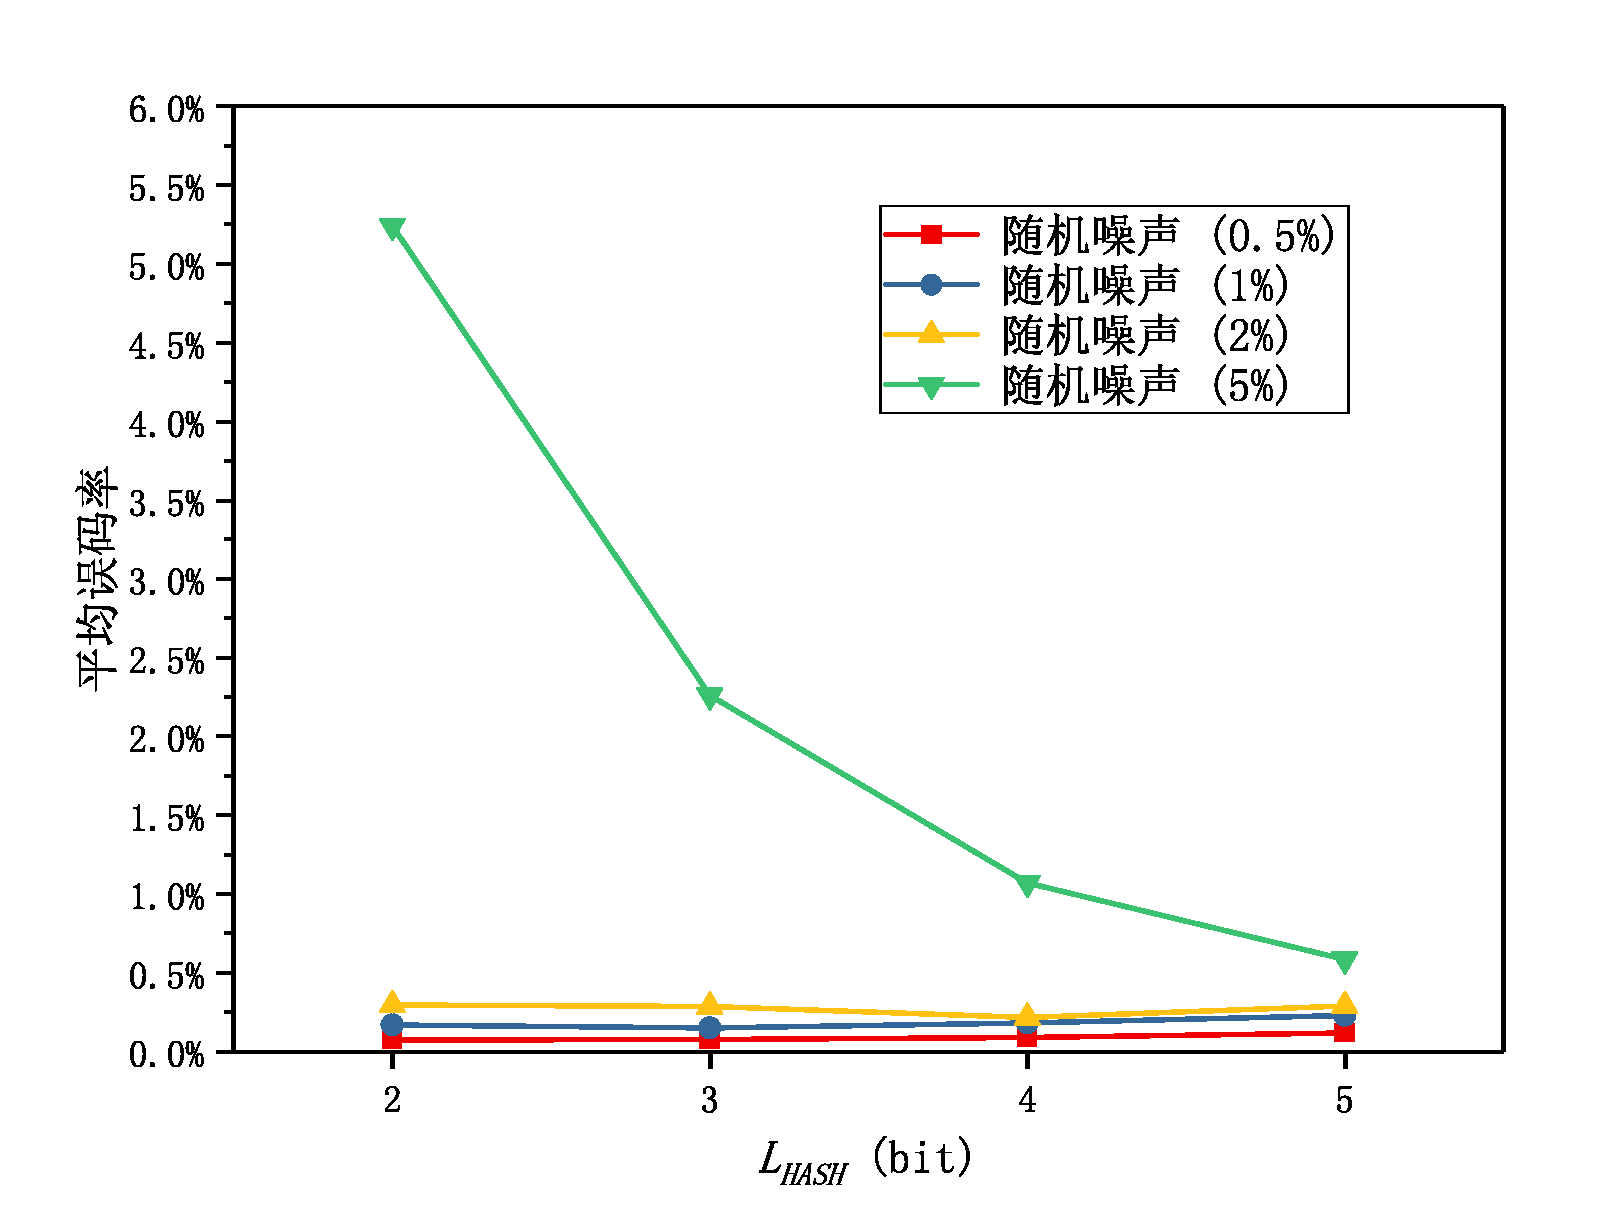
\includegraphics[width=0.48\textwidth]{chapters/chapter5/figures/ber-lhash-random.pdf}
        }
        \subfigure[$L_{CRC}$与平均误码率]{
            \label{fig:5:result:ber:random:lcrc}
            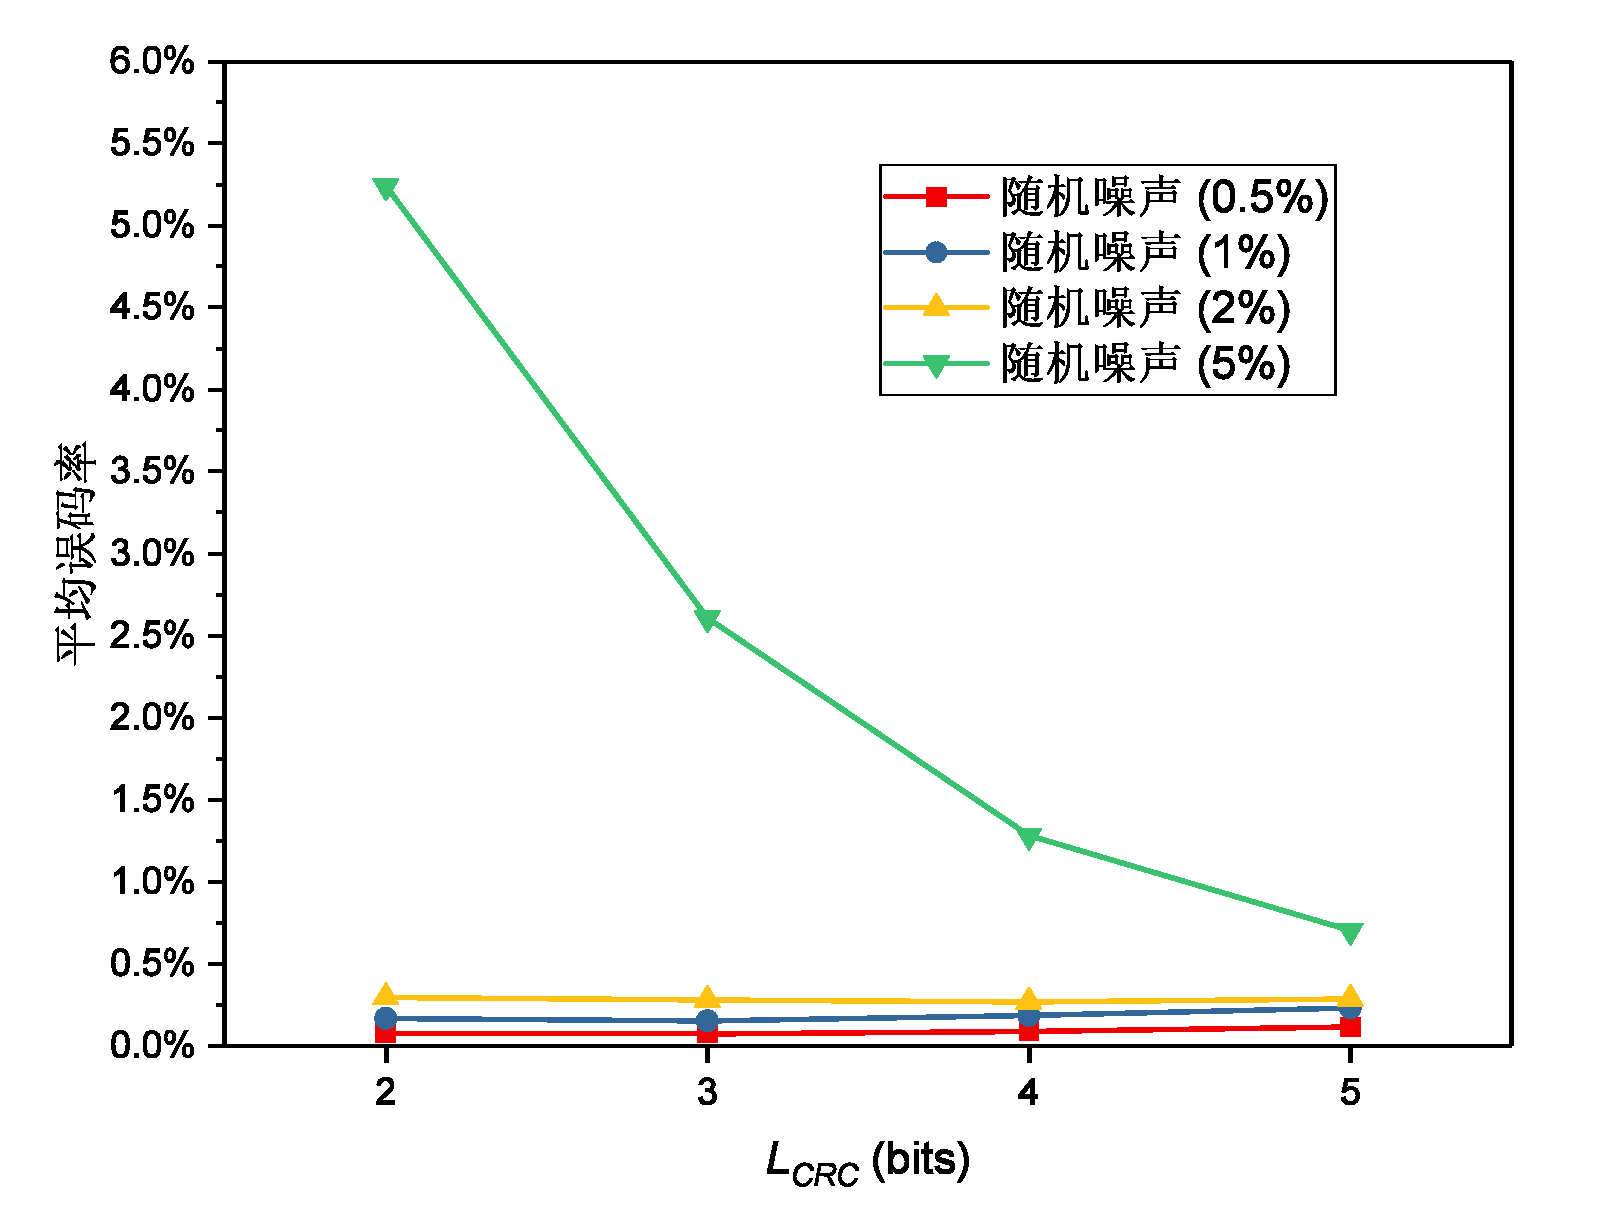
\includegraphics[width=0.48\textwidth]{chapters/chapter5/figures/ber-lcrc-random.pdf}
        }
        \subfigure[$R$与平均误码率]{
            \label{fig:5:result:ber:random:r}
            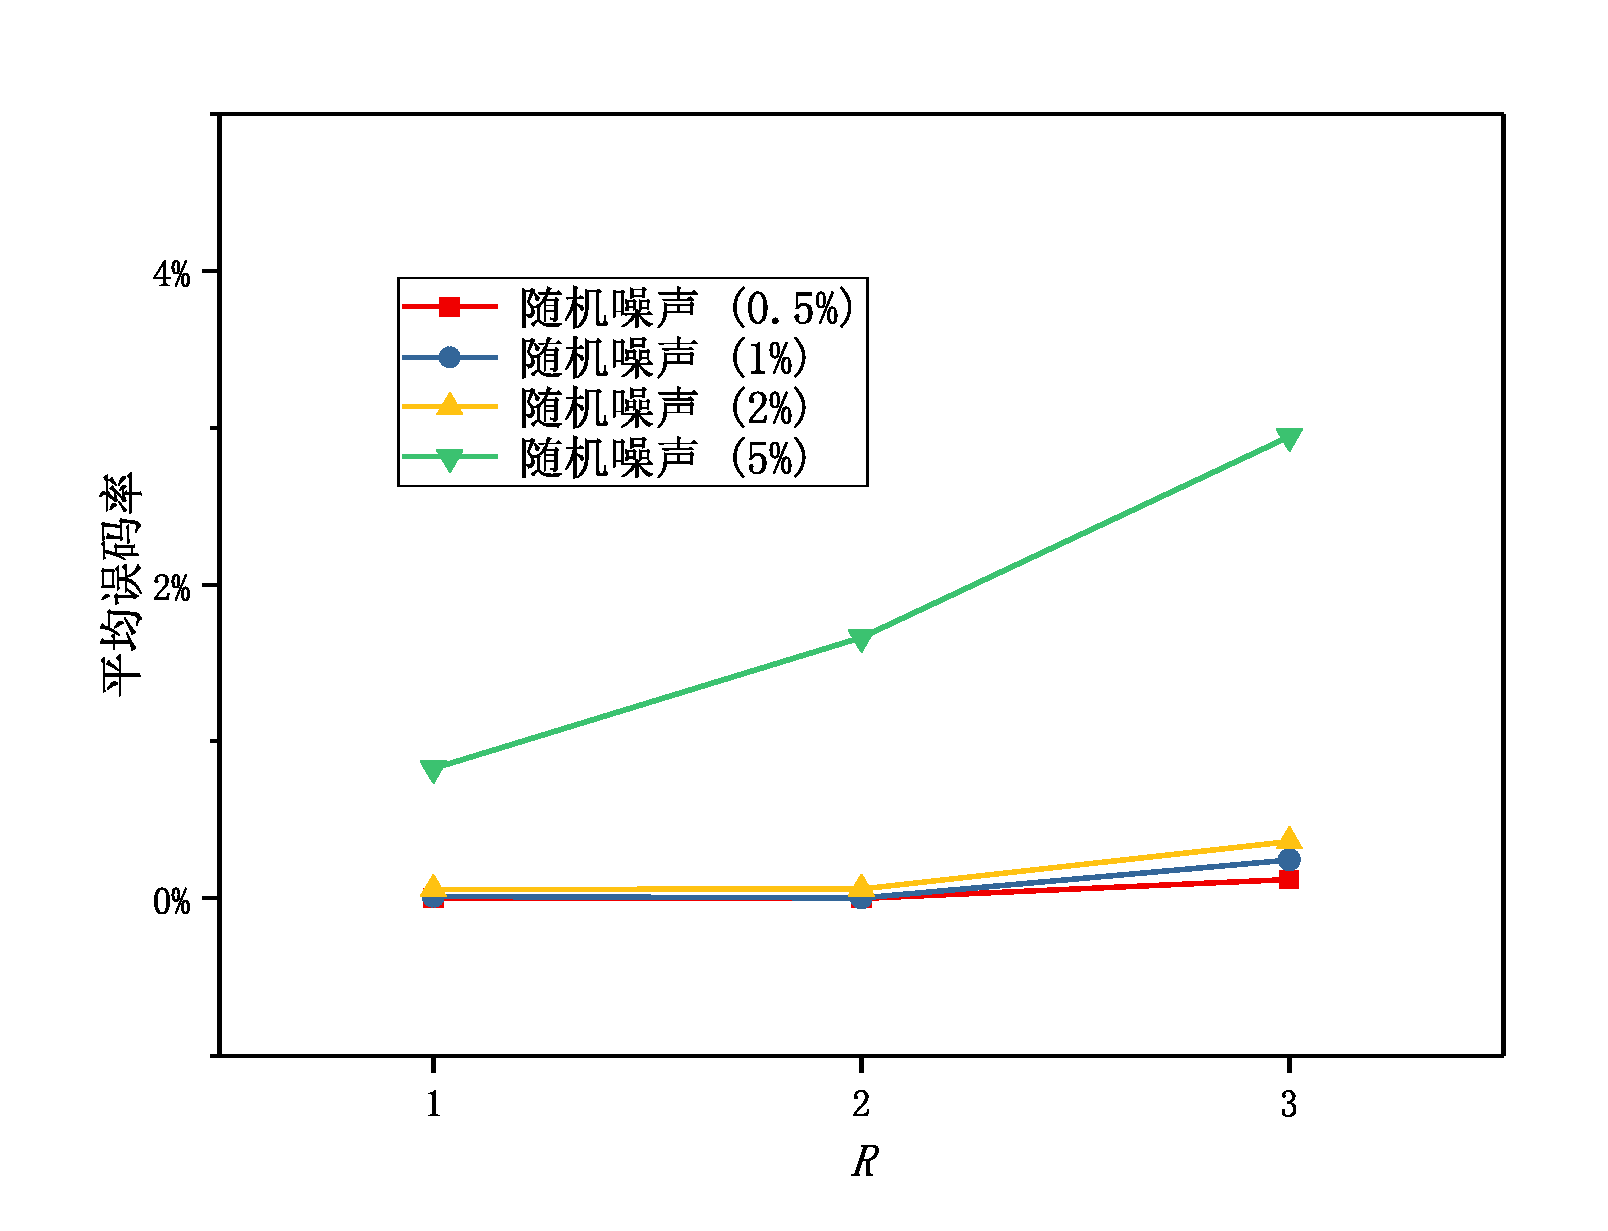
\includegraphics[width=0.48\textwidth]{chapters/chapter5/figures/ber-r-random.pdf}
        }
        \caption{随机噪声场景中平均误码率与传输参数的折线图}
        \label{fig:5:result:ber:random}
    \end{figure}
}

在随机噪声场景中,鲁棒性测试结果如图\nref{fig:5:result:ber:random}。由于该时间隐通道中存在多级校验,包括映射矩阵中基于异或的符号校验,已经能够对噪声进行有效拦截。因此在图\nref{fig:5:result:ber:random}中,当随机丢包率小于$2\%$时,平均误码率对随机丢包率的增长不敏感。在随机丢包噪声为$5\%$时,平均误码率曲线随参数变化出现明显波动,总体来说,减小$L_{Codeword}$、增大$L_{HASH}$、增大$L_{CRC}$及减小$R$均是有利于降低误码率的措施。

通过两种不同模式下的验证,通过调整该时间隐通道的设计参数,Excellent场景下误码率能够降低至$0.1\%$,Good场景下误码率能够降低至$5\%$。对于该时间隐通道的传输参数,增大$M_{cols}$、减小$L_{Codeword}$、增大$L_{HASH}$、增大$L_{CRC}$及减小$R$均可以降低误码率。根据公式(\nref{equ:5:codeword-length}),每个码字中含有的数据位数$BL$,与码字长度$L_{Codeword}$、HASH校验位数$L_{HASH}$及CRC校验位数$L_{CRC}$存在密切关系,提高鲁棒性对抗检测性及传输性能均产生一定影响,合适的参数配置需要综合考虑。

\subsection{传输性能测试}
\label{chap:hash:result:throughput}

根据该时间隐通道的设计方案,传输参数$L_{Codeword}$、$L_{HASH}$、$L_{CRC}$及$R$均影响传输性能。时间隐通道容量与参数的关系如公式(\nref{equ:5:capacity}),时间隐通道传输速率与参数的关系如公式(\nref{equ:5:throughput})。

\insertEquation{
    \begin{equation}
    \label{equ:5:capacity}
		Capacity\ =\ \frac{BL\ \times\ R}{(R\ +\ 1)\ \times\ 2^{L_{Codeword}}}\ (bpp)\ =\ \frac{(L_{Codeword}\ -\ L_{HASH}\ -\ L_{CRC})\ \times\ R}{(R\ +\ 1)\ \times\ 2^{L_{Codeword}}}\ (bpp)
    \end{equation}
    \begin{equation}
    \label{equ:5:throughput}
        Throughput\ =\ Capacity\ \times\ 100\ (bps)\ =\ \frac{(L_{Codeword}\ -\ L_{HASH}\ -\ L_{CRC})\ \times\ R}{(R\ +\ 1)\ \times\ 2^{L_{Codeword}}}\ (bps)
    \end{equation}
}

\insertFigure{
	\begin{figure}
        \centering
        \subfigure[$L_{HASH}+L_{CRC}=4$时的传输速率]{
            \label{fig:5:result:bps-4}
            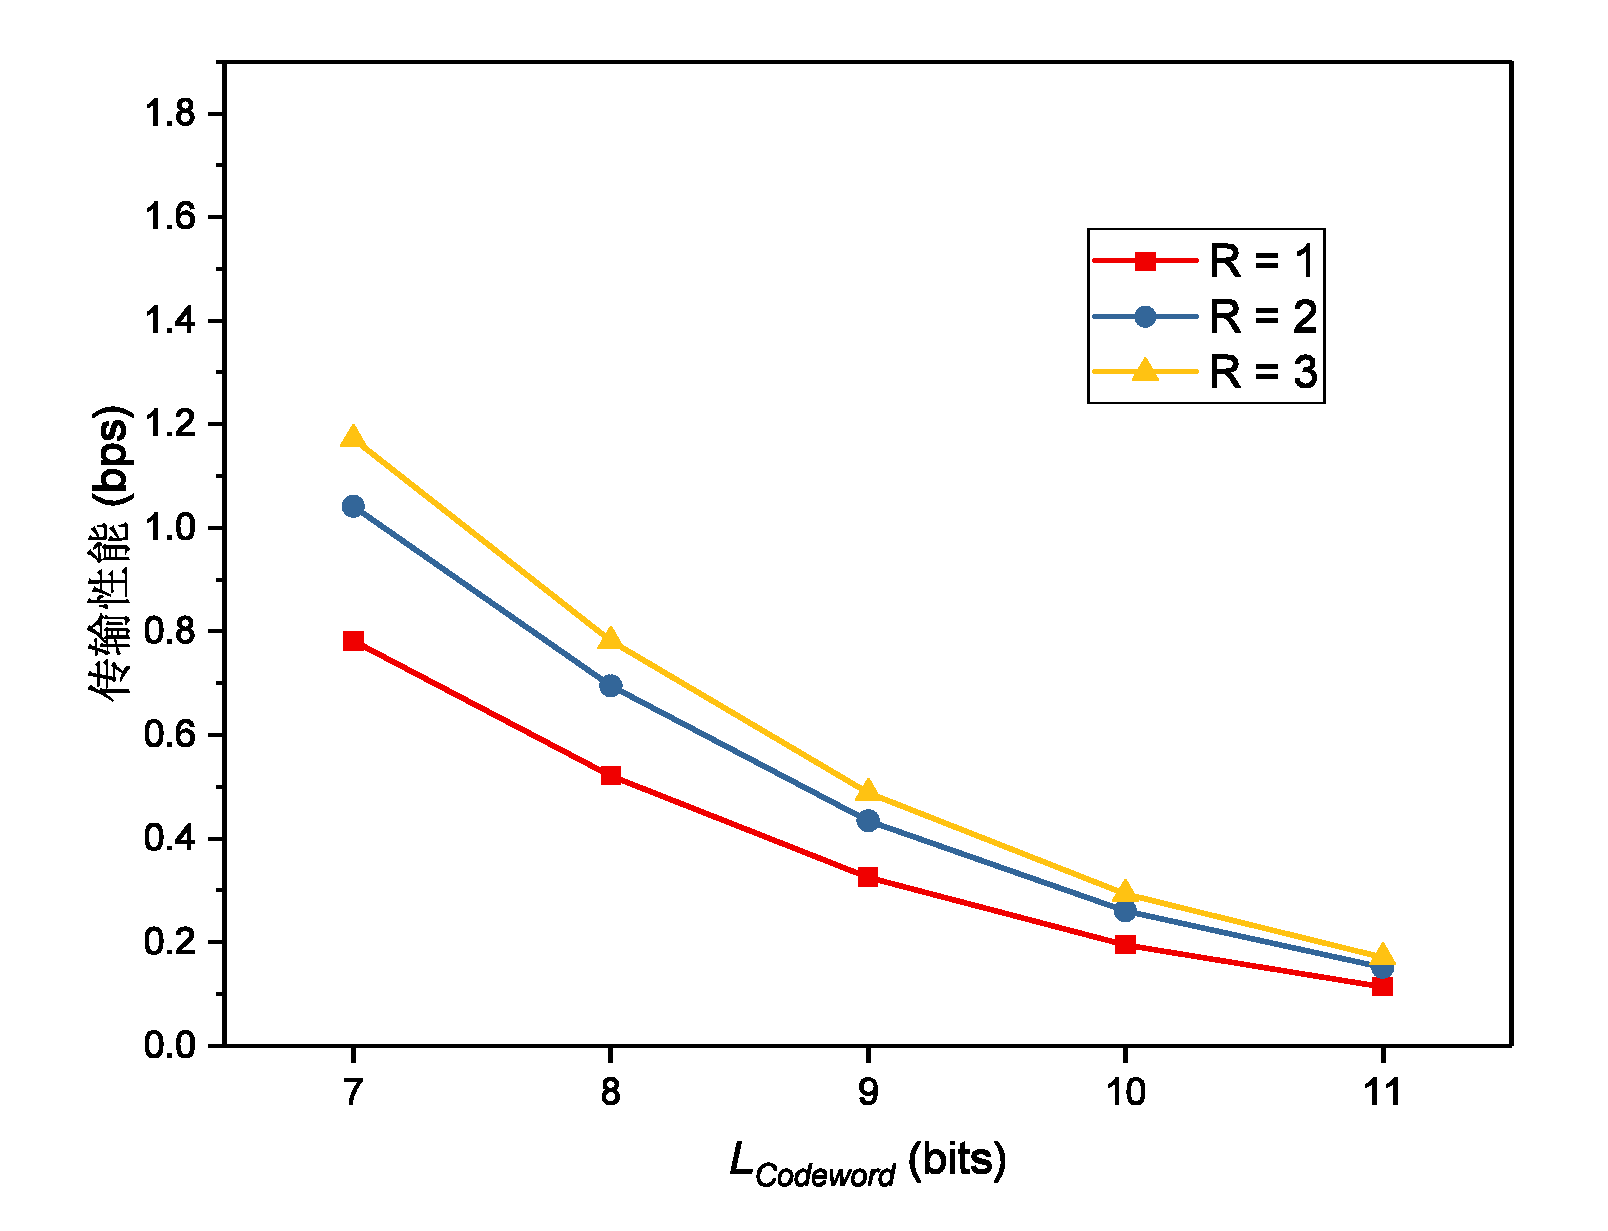
\includegraphics[width=0.48\textwidth]{chapters/chapter5/figures/bps-4.pdf}
        }
        \subfigure[$L_{HASH}+L_{CRC}=6$时的传输速率]{
            \label{fig:5:result:bps-6}
            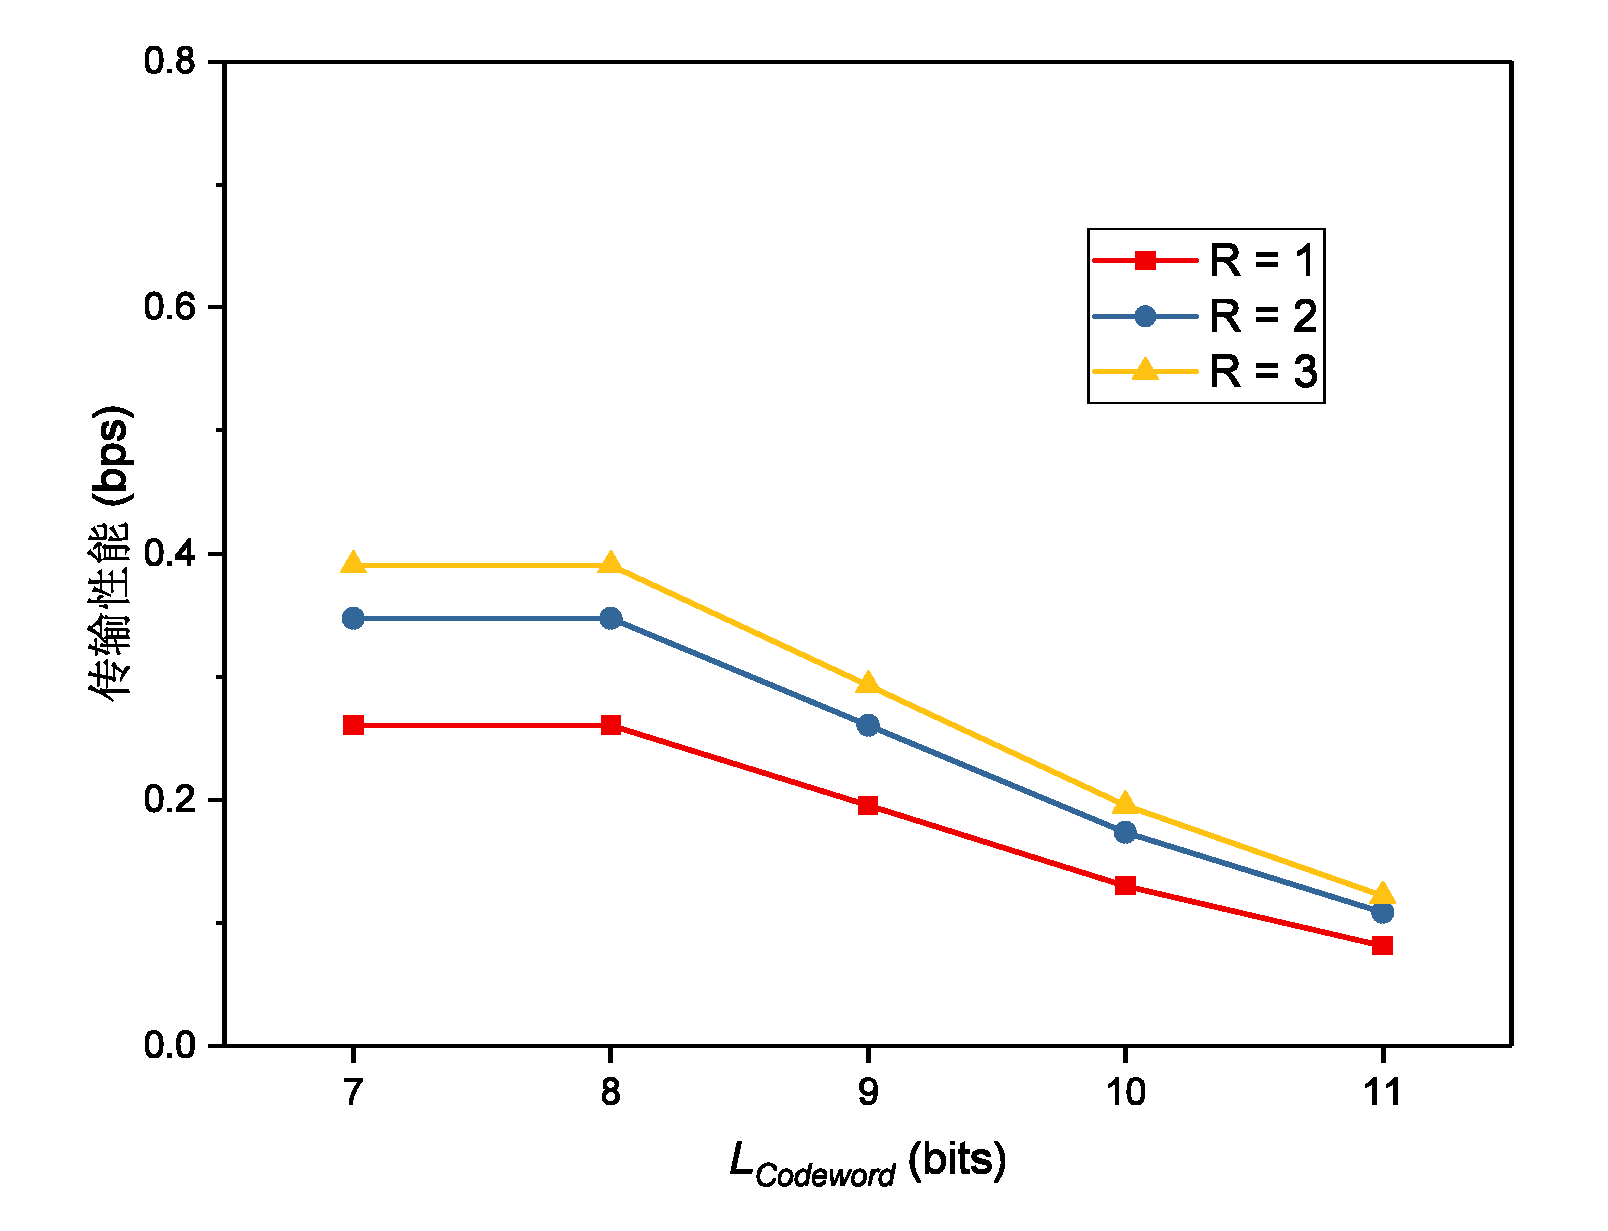
\includegraphics[width=0.48\textwidth]{chapters/chapter5/figures/bps-6.pdf}
        }
        \caption{时间隐通道的传输速率与$L_{Codeword}$与$R$的关系曲线}
        \label{fig:5:result:bps}
    \end{figure}
}

在$L_{HASH}+L_{CRC}=4$的模式下,时间隐通道的传输速率与$L_{Codeword}$及$R$的关系如图\nref{fig:5:result:bps-4}。在$L_{HASH}+L_{CRC}=6$的模式下,时间隐通道的传输速率与$L_{Codeword}$及$R$的关系如图\nref{fig:5:result:bps-6}。在Excellent场景中,传输性能可以达到{1.0\ bps}。通过增大复位周期$R$,在一定水平上提升传输速率,但远小于降低$L_{HASH}+L_{CRC}$带来的性能提升。

\subsection{构建代价测试}
\label{chap:hash:result:cost}

\insertFigure{
	\begin{figure}
        \centering
        \subfigure[Excellent场景的视频质量]{
            \label{fig:5:result:vq-excellent}
            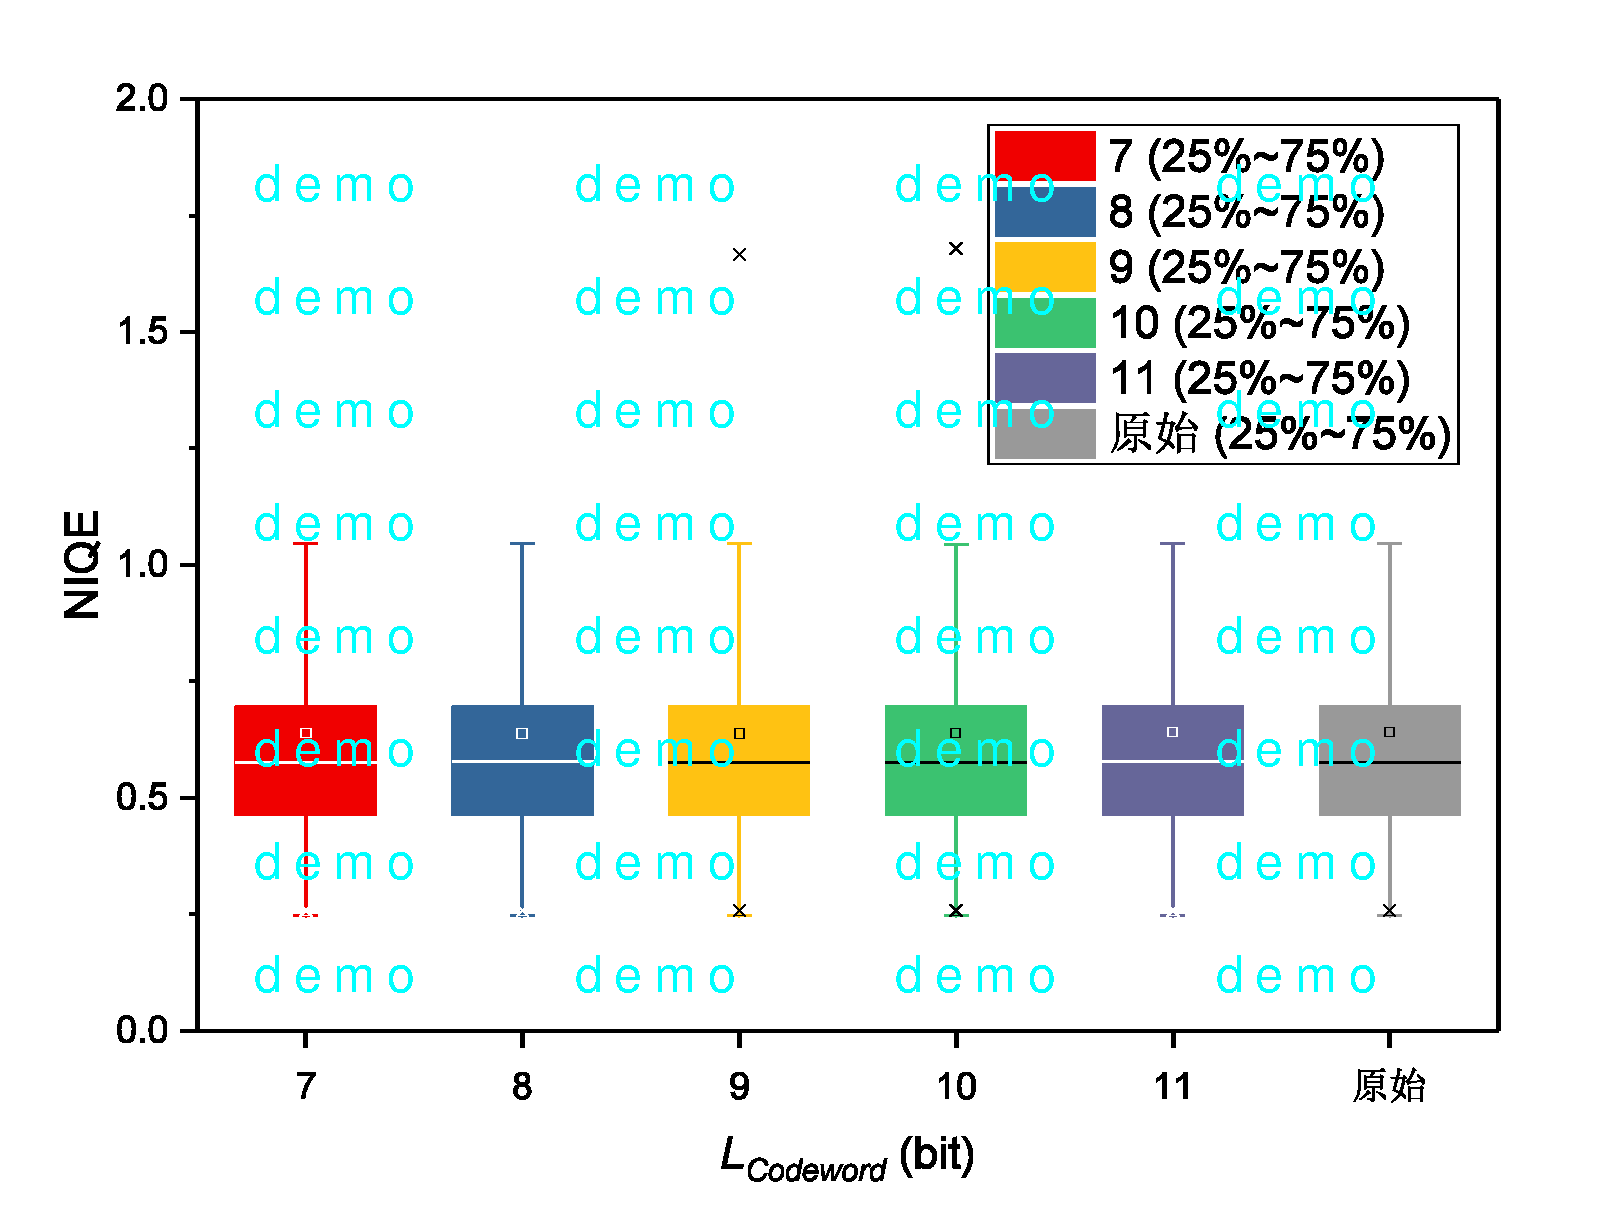
\includegraphics[width=0.48\textwidth]{chapters/chapter5/figures/vq-excellent.pdf}
        }
        \subfigure[Good场景的视频质量]{
            \label{fig:5:result:vq-good}
            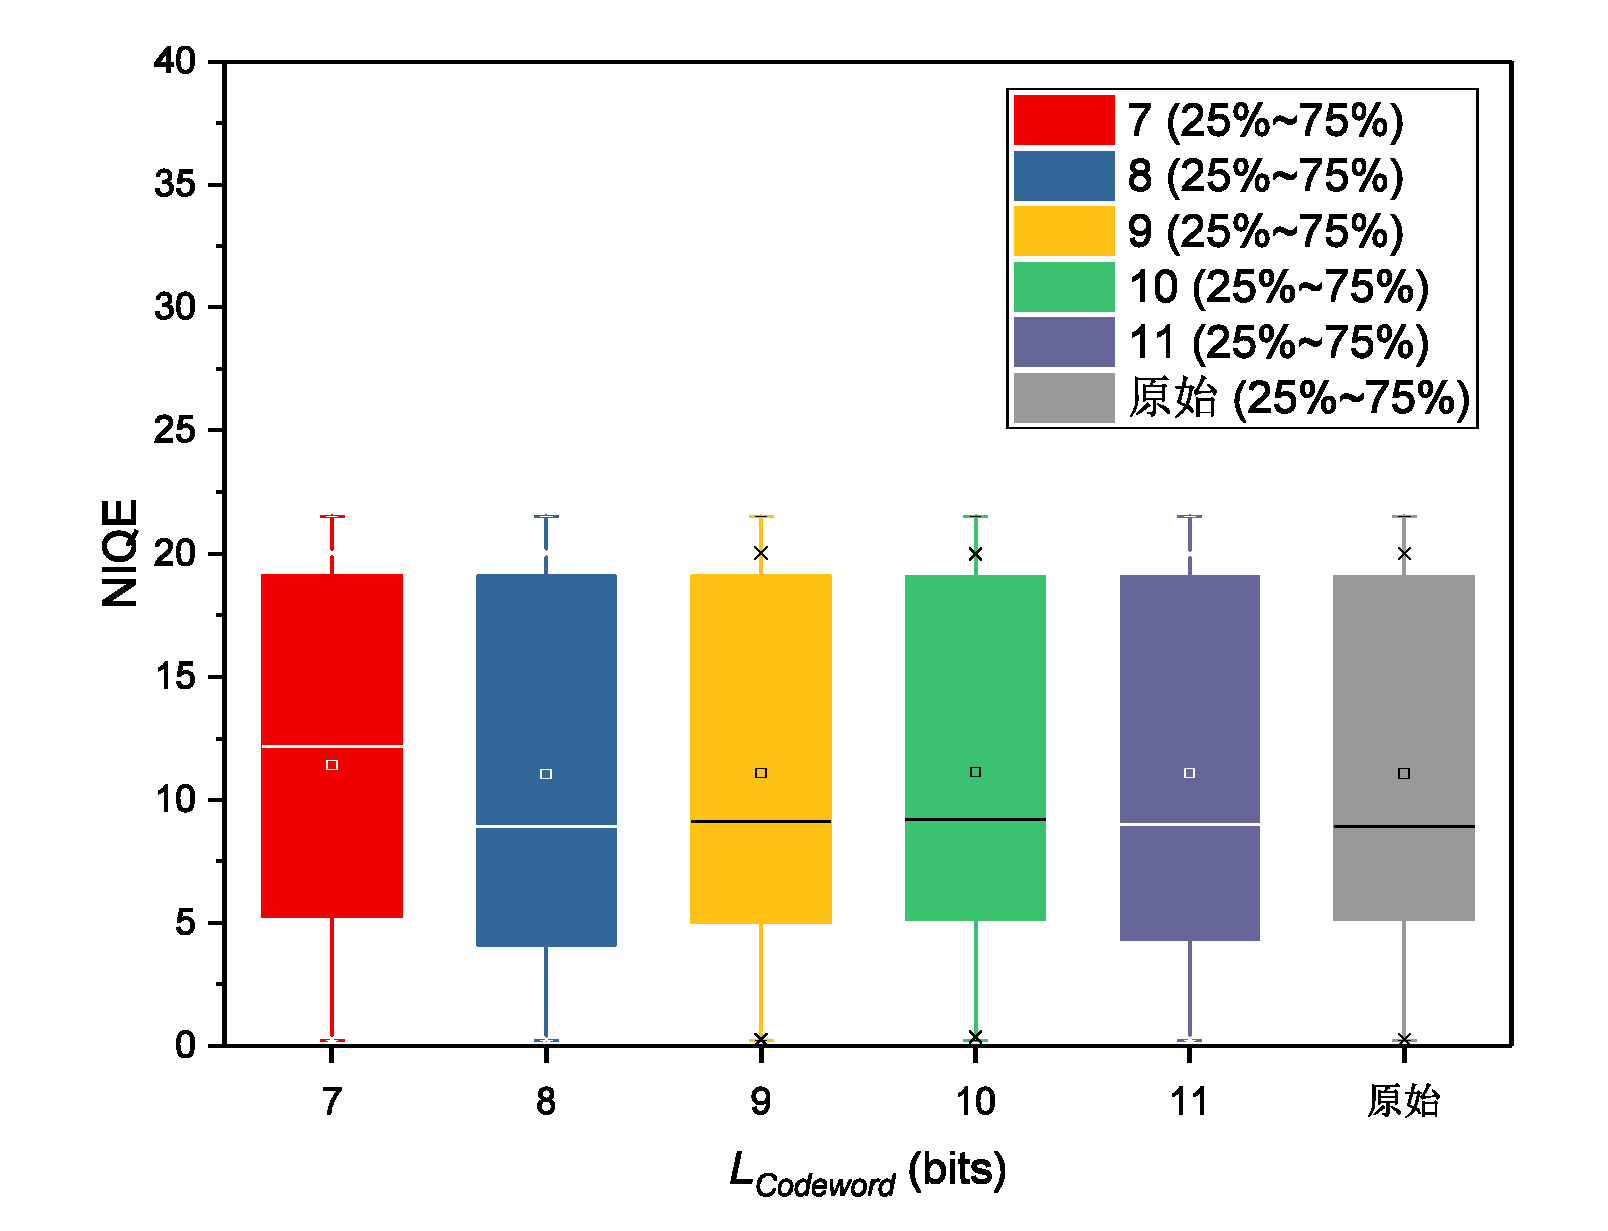
\includegraphics[width=0.48\textwidth]{chapters/chapter5/figures/vq-good.pdf}
        }
        \caption{时间隐通道的NIQE视频质量评估结果}
        \label{fig:5:result:vq}
    \end{figure}
}

该时间隐通道的构建代价测试,主要评估时间隐通道对视频质量的影响,评估指标采用NIQE(Natural Image Quality Evaluator)无参照质量指标\nupcite{7094273},较低的NIQE值对应较好的视频质量。时间隐通道的NIQE评估结果如图\nref{fig:5:result:vq},在两种场景中,由于网络噪声强度的差异,视频质量已经存在较大差异。图\nref{fig:5:result:vq-excellent},Excellent场景下,在不同$L_{Codeword}$下具有相似的NIQE值,且波动较小,时间隐通道对通话视频质量的影响可以忽略。图\nref{fig:5:result:vq-good},Good场景下,时间隐通道导致NIQE值产生波动,但无明显的分布差异。通过对比图\nref{fig:5:result:vq-excellent}及图\nref{fig:5:result:vq-good},相较构造时间隐通道导致的视频质量损失,网络噪声导致的视频质量损失更加明显,该时间隐通道对视频通话的影响可接受。

\subsection{测试结果汇总}
\label{chap:hash:result:evaluation}

通过测试该时间隐通道的抗检测性、鲁棒性、传输性能及构建代价,该方法中的多种传输参数对各方面表现有显著影响。在实际应用中,时间隐通道应当在保证传输隐蔽性的基础上,具有较好的鲁棒性和传输性能,因此,该时间隐通道的传输参数需要合理配置。根据\nref{chap:hash:result:undetectability}抗检测能力的测试结果,当$L_{Codeword}\ge 9$时,即可满足抗检测性的要求。时间隐通道作为寄生信道,受噪声干扰不可避免,通常在数据本身中结合其它鲁棒性方案保证传输可靠性,因此,在综合评估中,设定Excellent场景下平均误码率限定在$0.1\%$以内;Good场景下平均误码率限定在$1\%$以内。

\insertTable{
	\begin{table}
      \centering
      \caption{基于多重校验的时间隐通道参数组合评估表}
      \label{tab:5:result:results-sum}
          \begin{tabular*}{0.9\textwidth}{@{\extracolsep{\fill}}cccccccc}
            \toprule
            场景 & $M_{cols}$ & $L_{Codeword}$ & $L_{HASH}$ & $L_{CRC}$ & $R$ & 传输性能 & 平均误码率 \\
            \midrule
            \multirow{3}{*}{Excellent} 
            & 36 & 9 & 3 & 2 & 2 & 0.52\ bps & $<0.001\ \%$ \\
            & 27 & 9 & 2 & 3 & 3 & 0.59\ bps & $<0.02\ \%$ \\
            & 27 & 9 & 2 & 2 & 3 & 0.73\ bps & $<0.08\ \%$ \\
            \\
            \multirow{3}{*}{Good} 
            & 45 & 9 & 5 & 2 & 1 & 0.20\ bps & $<0.85\ \%$ \\
            & 36 & 10 & 5 & 3 & 3 & 0.15\ bps & $<0.1\ \%$ \\
            & 45 & 10 & 5 & 4 & 2 & 0.07\ bps & $<0.01\ \%$ \\
            \bottomrule
          \end{tabular*}
    \end{table}
}

该时间隐通道的综合评估表如表\nref{tab:5:result:results-sum},通过比较试验结果,分别选择出了Excellent场景及Good场景中的部分配置,这些配置参数在测试结果中具有较好的综合表现。由表可见Excellent场景下添加适当的鲁棒性信息,即可取得非常好的传输效果,在牺牲一定的鲁棒性时,能够取得更好的性能表现。Good场景中需要保持较多的鲁棒性信息,从而才能抵御噪声干扰,因此需要牺牲性能保证传输可靠性。

\insertTable{
	\begin{table}
      \centering
      \caption{基于多重校验的时间隐通道横向比较}
      \label{tab:5:result:compare}
          \begin{tabular*}{0.8\textwidth}{@{\extracolsep{\fill}}cccc}
            \toprule
            时间隐通道方法 & 传输性能 & 信道容量 & 误码率 \\
            \midrule
            SCC\nupcite{10.1007/978-3-642-16435-4_15} & & 0.2$\sim$ 0.8 bpp & 2\% \\
            AFTC\nupcite{7347395} & & 0.5 bpp & 4\% \\
            CoCo\nupcite{10.1007/978-3-642-24178-9_22} & & 0.1$\sim$ 0.5 bpp & 4\% \\
            SPCC\nupcite{8288828} & 0.7$\sim$ 3 bps & & 0.9\% \\
            Zigzag-CTC & 0.88 bps & 0.009 bpp & 1.5\% \\
            MSV-CTC & 0.73 bps & 0.007 bpp & 0.08\% \\
            \bottomrule
          \end{tabular*}
    \end{table}
}

表\nref{tab:5:result:compare}对比了几种时间隐通道的性能及误码率水平,分别为SCC\nupcite{10.1007/978-3-642-16435-4_15}、AFTC\nupcite{7347395}、CoCo\nupcite{10.1007/978-3-642-24178-9_22}、SPCC\nupcite{8288828}、基于Zigzag映射矩阵的时间隐通道Zigzag-CTC,及本时间隐通道构建方法MSV-CTC(Multi-Stage Verification Covert Timing Channel)。通过对比可以发现,虽然该时间隐通道损失了部分性能,但在鲁棒性方面有了显著提升,满足时间隐通道的设计要求。

\subsection{结论}
\label{chap:hash:result:conclusion}

通过抗检测能力测试、鲁棒性测试、传输性能测试及鲁棒性测试,该方法能够满足时间隐通道的指标要求,通过调整传输参数,能够在抗检测性、鲁棒性及传输性能间实现平衡。由于采用了主动丢包的调制方式,该时间隐通道在基于IPD的检测方法中具有较好的隐蔽性,并且调整参数$L_{Codeword}$后,可以通过突发丢包长度及区间丢包数的测试。

通过结合多个层次的数据校验方法,该时间隐通道有效提高了传输鲁棒性,误码率水平大幅降低。通过调整传输参数组合,在误码率水平$0.08\ \%$的情况下,具备0.73\ bps的传输性能,达到了时间隐通道基本水平。